\documentclass[12pt,a4paper]{article}

% --- Page Layout -------------------------------------------------------------
\usepackage[a4paper, top=0.8in, bottom=1.1in, left=0.8in, right=0.8in, headheight=14pt, footskip=30pt]{geometry}

% --- Fonts (XeLaTeX) ---------------------------------------------------------
\usepackage{fontspec}
\usepackage{unicode-math}
\setmainfont{TeX Gyre Pagella}
\setmonofont[Scale=0.88]{TeX Gyre Cursor}
\setmathfont{Latin Modern Math}

% --- Packages ---------------------------------------------------------------
\usepackage{xcolor}
\usepackage{titlesec}
\usepackage{enumitem}
\usepackage{tabularx}
\usepackage{booktabs}
\usepackage{array}
\usepackage{amsmath}
\usepackage{tikz}
\usetikzlibrary{shapes.geometric, arrows.meta, positioning, calc, fit, decorations.pathreplacing, decorations.pathmorphing}
\usepackage{tcolorbox}
\tcbuselibrary{skins, breakable}
\usepackage{hyperref}
\usepackage{fancyhdr}
\usepackage{graphicx}
\usepackage{microtype}
\hyphenpenalty=10000
\exhyphenpenalty=10000
\sloppy
\usepackage{caption}
\usepackage{setspace}
\usepackage{multirow}
\usepackage{tocloft}

% --- Q&A helper --------------------------------------------------------------
\newcommand{\Q}[1]{\textbf{#1}\par\noindent\ignorespaces}

% --- Colour Palette ----------------------------------------------------------
\definecolor{myred}{RGB}{196,30,58}
\definecolor{mydark}{RGB}{30,30,50}
\definecolor{mygreen}{RGB}{14,120,80}
\definecolor{myteal}{RGB}{0,130,140}
\definecolor{myamber}{RGB}{180,100,0}
\definecolor{mypurple}{RGB}{100,30,160}
\definecolor{mygray}{RGB}{246,247,249}
\definecolor{mgframe}{RGB}{180,185,200}
\definecolor{watermark}{RGB}{145,150,170}
\definecolor{hdrred}{RGB}{250,232,235}
\definecolor{hdrgreen}{RGB}{220,244,233}
\definecolor{hdrteal}{RGB}{220,242,244}
\definecolor{hdramber}{RGB}{253,242,215}
\definecolor{hdrpurple}{RGB}{238,228,255}
\definecolor{hdrgray}{RGB}{238,240,245}
\definecolor{rowalt}{RGB}{250,251,253}

% --- Section Formatting ------------------------------------------------------
\titleformat{\section}
  {\large\bfseries\color{myred}}{\thesection.}{0.5em}{}
  [\vspace{1pt}{\color{myred}\rule{\linewidth}{0.8pt}}]
\titleformat{\subsection}
  {\normalsize\bfseries\color{myteal}}{\thesubsection}{0.5em}{}
\titlespacing*{\section}{0pt}{18pt}{7pt}
\titlespacing*{\subsection}{0pt}{11pt}{4pt}

% --- Paragraph ---------------------------------------------------------------
\setlength{\parindent}{0pt}
\setlength{\parskip}{4pt}

% --- Page filling ------------------------------------------------------------
\raggedbottom

% --- TOC Styling -------------------------------------------------------------
\renewcommand{\cfttoctitlefont}{\large\bfseries\color{myred}}
\renewcommand{\cftaftertoctitle}{\par\noindent{\color{myred}\rule{\linewidth}{0.8pt}}}
\setlength{\cftbeforetoctitleskip}{0pt}
\setlength{\cftaftertoctitleskip}{6pt}
\renewcommand{\cftsecfont}{\normalsize\bfseries\color{mydark}}
\renewcommand{\cftsecpagefont}{\normalsize\bfseries\color{mydark}}
\renewcommand{\cftsecleader}{\cftdotfill{\cftdotsep}}
\setlength{\cftbeforesecskip}{7pt}
\renewcommand{\cftsubsecfont}{\small\color{mydark}}
\renewcommand{\cftsubsecpagefont}{\small\color{mydark}}
\setlength{\cftbeforesubsecskip}{3pt}
\setlength{\cftsubsecindent}{1.4em}

% --- Table helpers -----------------------------------------------------------
\renewcommand{\arraystretch}{1.45}
\setlength{\tabcolsep}{6pt}
\newcolumntype{B}[1]{>{\small\bfseries\raggedright\arraybackslash}m{#1}}
\newcolumntype{Y}{>{\small\raggedright\arraybackslash}X}
\renewcommand{\tabularxcolumn}[1]{m{#1}}

% --- Header / Footer ---------------------------------------------------------
\pagestyle{fancy}
\fancyhf{}
\fancyhead[L]{\small\color{myred}\textbf{BS-CH101}\;\color{mydark}--- Chemistry-I}
\fancyhead[R]{\small\color{myteal}\textbf{Module 5 Notes}}
\fancyfoot[L]{\small\color{watermark}\textit{\copyright\ MAKAUT Wingman}}
\fancyfoot[C]{\small\color{mydark}\thepage}
\fancyfoot[R]{\small\color{watermark}\textit{\copyright\ Biraj}}
\renewcommand{\headrulewidth}{0.5pt}
\renewcommand{\footrulewidth}{0.3pt}

% --- Hyperref ---------------------------------------------------------------
\hypersetup{
  colorlinks=true, linkcolor=myteal, urlcolor=myteal,
  pdfauthor={Biraj Sarkar},
  pdftitle={BS-CH101 --- Module 5 Long Notes: Periodic Properties}
}

% --- tcolorbox styles --------------------------------------------------------
\tcbset{
  tikzbox/.style={
    colback=mygray, colframe=mgframe, boxrule=0.6pt, arc=4pt,
    left=8pt, right=8pt, top=6pt, bottom=6pt,
    colbacktitle=mgframe, coltitle=mydark,
    fonttitle=\small\bfseries
  },
  defbox/.style={
    colback=hdrgreen, colframe=mygreen, boxrule=0.8pt, arc=4pt,
    left=9pt, right=9pt, top=6pt, bottom=6pt,
    colbacktitle=mygreen, coltitle=white,
    fonttitle=\small\bfseries
  },
  formulabox/.style={
    colback=hdrteal, colframe=myteal, boxrule=0.8pt, arc=4pt,
    left=9pt, right=9pt, top=7pt, bottom=7pt,
    colbacktitle=myteal, coltitle=white,
    fonttitle=\small\bfseries
  },
  examplebox/.style={
    colback=hdramber, colframe=myamber, boxrule=0.8pt, arc=4pt,
    left=9pt, right=9pt, top=6pt, bottom=6pt,
    colbacktitle=myamber, coltitle=white,
    fonttitle=\small\bfseries
  },
  masonbox/.style={
    colback=hdrpurple, colframe=mypurple, boxrule=0.8pt, arc=4pt,
    left=9pt, right=9pt, top=6pt, bottom=6pt,
    colbacktitle=mypurple, coltitle=white,
    fonttitle=\small\bfseries
  },
  exambox/.style={
    colback=hdrpurple, colframe=mypurple, boxrule=1pt, arc=5pt,
    left=10pt, right=10pt, top=8pt, bottom=8pt,
    colbacktitle=mypurple, coltitle=white,
    fonttitle=\bfseries, breakable, title after break={\textbf{Frequently Asked / Viva Questions (contd.)}}}
}
% --- TikZ styles -------------------------------------------------------------
\tikzset{
  block/.style={rectangle, draw=myteal, fill=hdrteal,
    text width=2.4cm, align=center, minimum height=0.95cm,
    font=\small, rounded corners=3pt, line width=0.7pt},
  redblock/.style={rectangle, draw=myred, fill=hdrred,
    text width=2.4cm, align=center, minimum height=0.95cm,
    font=\small, rounded corners=3pt, line width=0.7pt},
  netnode/.style={rectangle, draw=myteal, fill=hdrteal,
    text width=1.5cm, align=center, minimum height=0.8cm,
    font=\small, rounded corners=3pt, line width=0.7pt},
  sumjunc/.style={circle, draw=myamber, fill=hdramber,
    minimum size=0.62cm, font=\small, line width=0.8pt},
  snode/.style={circle, draw=mypurple, fill=hdrpurple,
    minimum size=0.55cm, font=\footnotesize, line width=0.7pt},
  arrow/.style={-Stealth, thick, color=mydark},
  redarrow/.style={-Stealth, thick, color=myred},
  line/.style={thick, color=mydark}
}

\tcbset{breakable}

\begin{document}

\begin{center}
  {\LARGE\bfseries\color{myred} BS-CH101 --- Chemistry-I}\\[5pt]
  {\normalsize\color{mydark} Semester I/II \quad$\bullet$\quad 3L:1T:0P \quad$\bullet$\quad 4 Credits}\\[3pt]
  {\normalsize\color{myteal}\textbf{Module 5 Exam Notes: Periodic Properties}}\\[3pt]
  {\small\color{mydark} CGEC \;$|$\; B.Tech ECE (2023--27) \;$|$\; \textit{Biraj Sarkar}}
\end{center}

\noindent{\color{myred}\rule{\linewidth}{1.2pt}}
\vspace{10pt}

\tableofcontents
\newpage

% =============================================================================
\section{Effective Nuclear Charge \& Slater's Rules}
% =============================================================================

\begin{tcolorbox}[defbox, title={Definitions: Shielding and Effective Nuclear Charge}]
  \textbf{Shielding (Screening) Effect:} The phenomenon where inner-shell electrons screen or shield valence-shell electrons from the electrostatic attraction of the positively charged nucleus.
  \par\vspace{4pt}
  \textbf{Effective Nuclear Charge ($Z_{\text{eff}}$):} The net positive charge experienced by an electron in a multi-electron atom. It is always less than the actual nuclear charge ($Z$) due to the shielding effect of other electrons.
\end{tcolorbox}

\subsection{Conceptual Framework}
In a hydrogenic atom (an atom with only one electron like $\text{H}$, $\text{He}^+$, or $\text{Li}^{2+}$), the electron experiences the full attraction of the nucleus of charge $+Ze$. The potential energy is simply:
\[ V(r) = -\frac{Ze^2}{4\pi\varepsilon_0 r} \]
However, in a multi-electron atom, any single electron experiences:
\begin{enumerate}
  \item The attractive electrostatic force from the positively charged nucleus.
  \item The repulsive electrostatic forces from all other electrons present in the atom.
\end{enumerate}

These electron-electron repulsions reduce the net attraction of the nucleus on the electron. Conceptually, we can view the valence electron as experiencing a spherically averaged cloud of negative charge formed by the inner electrons, which partially cancels the positive nuclear charge. The nuclear charge that the outer electron actually feels is the \textbf{Effective Nuclear Charge ($Z_{\text{eff}}$)}, defined quantitatively as:

\begin{tcolorbox}[formulabox, title={Effective Nuclear Charge Equation}]
  \[ Z_{\text{eff}} = Z - \sigma \]
  Where:
  \begin{itemize}[leftmargin=1.5cm, itemsep=1pt]
    \item[$Z$] = Actual atomic number (number of protons in the nucleus).
    \item[$\sigma$] = Shielding (screening) constant, representing the total shielding capability of all other electrons.
  \end{itemize}
\end{tcolorbox}

\subsection{Slater's Rules for Estimating \texorpdfstring{$\sigma$}{sigma}}
John C. Slater proposed a set of semi-empirical rules in 1930 to estimate the shielding constant ($\sigma$) for any electron in an atom. To apply Slater's rules, the electrons of the atom are grouped in a specific sequence, and different shielding values are assigned based on the orbital type and shell level.

\textbf{Step 1: Write the Electronic Configuration in Groups}
Write the electronic configuration of the atom in the following order and grouping:
\[ (1s) \; (2s, 2p) \; (3s, 3p) \; (3d) \; (4s, 4p) \; (4d) \; (4f) \; (5s, 5p) \; (5d) \dots \]
Notice that $s$ and $p$ orbitals of the same principal quantum number ($n$) are grouped together, whereas $d$ and $f$ orbitals are kept in their own separate groups.

\textbf{Step 2: Rules for $s$ or $p$ Valence Electrons}
For an electron residing in an $(ns, np)$ group, the screening constant $\sigma$ is calculated by summing the contributions from all other electrons in the atom:
\begin{itemize}[leftmargin=*, itemsep=2pt]
  \item \textbf{Electrons in groups to the right:} Contribute \textbf{0} to $\sigma$ (higher shells do not shield inner shells).
  \item \textbf{Electrons in the same $(ns, np)$ group:} Contribute \textbf{0.35} each (except for the $1s$ group, where the other electron shields by \textbf{0.30}).
  \item \textbf{Electrons in the $(n-1)$ shell (penultimate shell):} Contribute \textbf{0.85} each.
  \item \textbf{Electrons in the $(n-2)$ and deeper shells (inner core):} Contribute \textbf{1.00} each.
\end{itemize}

\textbf{Step 3: Rules for $d$ or $f$ Valence Electrons}
For an electron residing in an $(nd)$ or $(nf)$ group:
\begin{itemize}[leftmargin=*, itemsep=2pt]
  \item \textbf{Electrons in groups to the right:} Contribute \textbf{0} to $\sigma$.
  \item \textbf{Electrons in the same $(nd)$ or $(nf)$ group:} Contribute \textbf{0.35} each.
  \item \textbf{Electrons in all groups to the left (inner shells):} Contribute \textbf{1.00} each.
\end{itemize}
This means that for $d$ and $f$ electrons, all electrons in lower energy groups (including $s$ and $p$ electrons of the same principal quantum number $n$ if they are to the left, e.g., $3s, 3p$ for a $3d$ electron) shield completely with a factor of $1.00$.

\subsection{Worked Examples of Slater's Calculations}

\begin{tcolorbox}[examplebox, title={Example 1.1: Calculation for Carbon ($C$, $Z=6$)}]
  Determine $Z_{\text{eff}}$ experienced by a valence ($2p$) electron in a ground-state Carbon atom.
  \par\vspace{4pt}
  \textbf{Solution:}
  \begin{enumerate}
    \item Group the configuration: $(1s^2) \; (2s^2, 2p^2)$.
    \item We target one electron in the valence group $(2s, 2p)$. The remaining electrons in this group is: $(2 + 2 - 1) = 3$ electrons.
    \item The inner group $(1s)$ contains 2 electrons.
    \item Calculate $\sigma$:
      \[ \sigma = (3 \times 0.35) + (2 \times 0.85) = 1.05 + 1.70 = 2.75 \]
    \item Calculate $Z_{\text{eff}}$:
      \[ Z_{\text{eff}} = Z - \sigma = 6 - 2.75 = 3.25 \]
  \end{enumerate}
  Therefore, a valence electron in Carbon feels an effective positive charge of $+3.25e$ instead of the full nuclear charge $+6e$.
\end{tcolorbox}

\begin{tcolorbox}[examplebox, title={Example 1.2: Calculation for Iron ($Fe$, $Z=26$)}]
  Compare the effective nuclear charge ($Z_{\text{eff}}$) experienced by:
  \begin{enumerate}[label=(\alph*), itemsep=1pt, topsep=2pt]
    \item A valence $4s$ electron in Iron.
    \item A $3d$ electron in Iron.
  \end{enumerate}
  \par\vspace{4pt}
  \textbf{Solution:}
  The electronic configuration is $1s^2 2s^2 2p^6 3s^2 3p^6 3d^6 4s^2$.
  Grouping: $(1s^2) \; (2s^2, 2p^6) \; (3s^2, 3p^6) \; (3d^6) \; (4s^2)$.
  \par\vspace{4pt}
  \textbf{(a) Calculation for a $4s$ electron ($n=4$):}
  \begin{itemize}[leftmargin=*, itemsep=2pt]
    \item Electrons in same group ($4s$): $2 - 1 = 1$ electron (contributes $0.35$).
    \item Electrons in $n-1$ shell ($3s, 3p, 3d$): $2 + 6 + 6 = 14$ electrons (contribute $0.85$ each).
    \item Electrons in $n-2$ and deeper shells ($1s, 2s, 2p$): $2 + 2 + 6 = 10$ electrons (contribute $1.00$ each).
  \end{itemize}
  \[ \sigma_{4s} = (1 \times 0.35) + (14 \times 0.85) + (10 \times 1.00) = 0.35 + 11.90 + 10.00 = 22.25 \]
  \[ Z_{\text{eff}, 4s} = Z - \sigma_{4s} = 26 - 22.25 = 3.75 \]
  \par\vspace{4pt}
  \textbf{(b) Calculation for a $3d$ electron ($n=3$):}
  Since we are targeting a $3d$ electron, the outer $(4s^2)$ group is to the right and contributes $0$.
  \begin{itemize}[leftmargin=*, itemsep=2pt]
    \item Electrons in same group ($3d$): $6 - 1 = 5$ electrons (contribute $0.35$ each).
    \item Electrons in groups to the left ($1s, 2s, 2p, 3s, 3p$): $2 + 2 + 6 + 2 + 6 = 18$ electrons (contribute $1.00$ each).
  \end{itemize}
  \[ \sigma_{3d} = (5 \times 0.35) + (18 \times 1.00) = 1.75 + 18.00 = 19.75 \]
  \[ Z_{\text{eff}, 3d} = Z - \sigma_{3d} = 26 - 19.75 = 6.25 \]
  \par\vspace{4pt}
  \textbf{Conclusion:} The $3d$ electrons feel a much stronger effective nuclear charge ($6.25$) than the $4s$ electrons ($3.75$). This is why $4s$ electrons, despite being filled first in neutral atoms according to the Aufbau heuristic, are the first to be ionized when forming transition-metal cations (e.g., $\text{Fe}^{2+}$ is $[\text{Ar}]3d^6$, not $[\text{Ar}]3d^4 4s^2$).
\end{tcolorbox}

\begin{tcolorbox}[examplebox, title={Example 1.3: Calculation for Zinc ($Zn$, $Z=30$)}]
  Calculate the $Z_{\text{eff}}$ experienced by:
  \begin{enumerate}[label=(\alph*), itemsep=1pt, topsep=2pt]
    \item A valence $4s$ electron in Zinc.
    \item A $3d$ electron in Zinc.
  \end{enumerate}
  \par\vspace{4pt}
  \textbf{Solution:}
  Grouping: $(1s^2) \; (2s^2, 2p^6) \; (3s^2, 3p^6) \; (3d^{10}) \; (4s^2)$.
  \par\vspace{4pt}
  \textbf{(a) Calculation for a $4s$ electron ($n=4$):}
  \begin{itemize}[leftmargin=*, itemsep=1pt]
    \item Same group ($4s$): $2 - 1 = 1$ electron $\times 0.35 = 0.35$.
    \item $n-1$ shell ($3s, 3p, 3d$): $(2 + 6 + 10) = 18$ electrons $\times 0.85 = 15.30$.
    \item $n-2$ and inner shells ($1s, 2s, 2p$): $10$ electrons $\times 1.00 = 10.00$.
  \end{itemize}
  \[ \sigma_{4s} = 0.35 + 15.30 + 10.00 = 25.65 \]
  \[ Z_{\text{eff}, 4s} = 30 - 25.65 = 4.35 \]
  \par\vspace{4pt}
  \textbf{(b) Calculation for a $3d$ electron ($n=3$):}
  Ignore $(4s^2)$ to the right.
  \begin{itemize}[leftmargin=*, itemsep=1pt]
    \item Same group ($3d$): $10 - 1 = 9$ electrons $\times 0.35 = 3.15$.
    \item Inner groups to the left: $18$ electrons $\times 1.00 = 18.00$.
  \end{itemize}
  \[ \sigma_{3d} = 3.15 + 18.00 = 21.15 \]
  \[ Z_{\text{eff}, 3d} = 30 - 21.15 = 8.85 \]
\end{tcolorbox}

\subsection{Trends in Effective Nuclear Charge}
Across a period, as we move from left to right:
\begin{itemize}[leftmargin=*, itemsep=2pt]
  \item The atomic number ($Z$) increases by 1 unit per element.
  \item The valence electrons are added to the same principal shell, which shields other valence electrons very poorly ($\sigma$ increases by only $0.35$).
  \item Consequently, the effective nuclear charge ($Z_{\text{eff}}$) increases steadily by approximately $0.65$ with each successive element:
  \[ \Delta Z_{\text{eff}} = \Delta Z - \Delta\sigma = 1 - 0.35 = 0.65 \]
\end{itemize}
This steady increase in $Z_{\text{eff}}$ across a period pulls the electron cloud closer to the nucleus, causing atomic sizes to decrease, and ionization energies to increase.

Down a group, as we move from top to bottom:
\begin{itemize}[leftmargin=*, itemsep=2pt]
  \item New electronic shells are added.
  \item Although the actual nuclear charge $Z$ increases dramatically, the inner shell electrons screen the nucleus very effectively.
  \item Using Slater's rules, $Z_{\text{eff}}$ remains relatively constant or increases only slightly for valence electrons down a group. For instance:
    \begin{itemize}
      \item $\text{Li}$: $Z_{\text{eff}} = 3 - (2 \times 0.85) = 1.30$.
      \item $\text{Na}$: $Z_{\text{eff}} = 11 - (8 \times 0.85 + 2 \times 1.00) = 11 - 8.80 = 2.20$.
      \item $\text{K}$: $Z_{\text{eff}} = 19 - (8 \times 0.85 + 10 \times 1.00) = 19 - 16.80 = 2.20$.
    \end{itemize}
\end{itemize}

\begin{tcolorbox}[exambox, title={Exam Points: Effective Nuclear Charge}]
  \begin{itemize}[leftmargin=*, itemsep=2pt, topsep=2pt]
    \item \textbf{Slater's Grouping:} Remember to group $s$ and $p$ together, but keep $d$ and $f$ separate.
    \item \textbf{Differentiation:} $d$ and $f$ electrons do not shield other electrons in the same shell as well as $s/p$ do, resulting in higher $Z_{\text{eff}}$ for $d$ orbitals.
    \item \textbf{Transition metal ionization:} Explain why $\text{Fe}^{2+}$ forms by losing $4s$ rather than $3d$ electrons using calculated $Z_{\text{eff}}$ ($Z_{\text{eff}, 4s} = 3.75$ vs. $Z_{\text{eff}, 3d} = 6.25$).
    \item \textbf{Periodic trends:} $Z_{\text{eff}}$ increases by $0.65$ per element across a period, which is the primary driver behind periodic contractions in atomic radii.
  \end{itemize}
\end{tcolorbox}

% =============================================================================
\section{Penetration of Orbitals \& Orbital Energies}
% =============================================================================

\begin{tcolorbox}[defbox, title={Definitions: Penetration and Radial Nodes}]
  \textbf{Penetration:} The ability of an orbital to attract electron density close to the nucleus. An electron in a highly penetrating orbital experiences less shielding and feels a higher effective nuclear charge ($Z_{\text{eff}}$).
  \par\vspace{4pt}
  \textbf{Radial Node (Spherical Node):} A spherical region where the probability of finding an electron is zero. The number of radial nodes for any orbital is given by:
  \[ N_r = n - l - 1 \]
  Where $n$ is the principal quantum number and $l$ is the azimuthal quantum number.
\end{tcolorbox}

\subsection{Orbital Penetration and Radial Distribution Functions}
To understand why orbitals of the same principal quantum number $n$ have different energies in a multi-electron atom, we must analyze their radial probability density distributions. The radial distribution function $P(r) = 4\pi r^2 R_{nl}(r)^2$ represents the probability of finding the electron in a spherical shell of radius $r$ and thickness $dr$ around the nucleus.

For a given principal shell $n$, the azimuthal quantum number $l$ determines the shape and the number of nodes of the orbital. As $l$ increases, the orbital angular momentum increases, creating a centrifugal barrier that keeps the electron away from the nucleus. Consequently:
\begin{itemize}[leftmargin=*, itemsep=2pt]
  \item \textbf{$s$ orbitals ($l=0$):} Have the maximum probability density close to the nucleus ($r \to 0$). They have $(n-1)$ radial nodes, which means they contain small inner peaks of electron density very close to the nucleus.
  \item \textbf{$p$ orbitals ($l=1$):} Have less density near the nucleus than $s$ orbitals. They have $(n-2)$ radial nodes.
  \item \textbf{$d$ orbitals ($l=2$):} Have very low density near the nucleus. They have $(n-3)$ radial nodes.
  \item \textbf{$f$ orbitals ($l=3$):} Have virtually zero density near the nucleus, behaving as diffuse shells.
\end{itemize}

This ability of an electron in a given orbital to spend time close to the nucleus, passing through the inner shell electron cloud, is called \textbf{penetration}. For any given principal shell $n$, the penetration power decreases in the order:

\begin{tcolorbox}[formulabox, title={Penetration Power Trend}]
  \[ s > p > d > f \]
\end{tcolorbox}

Because an $s$ electron penetrates the inner core electrons more effectively than $p, d$, or $f$ electrons of the same shell, it is shielded less. Consequently, the $s$ electron experiences a higher effective nuclear charge ($Z_{\text{eff}}$), is bound more tightly to the nucleus, and resides at a lower energy level.

\begin{tcolorbox}[tikzbox, title={Radial Probability Distribution Curves for $n=3$ Orbitals}]
\begin{center}
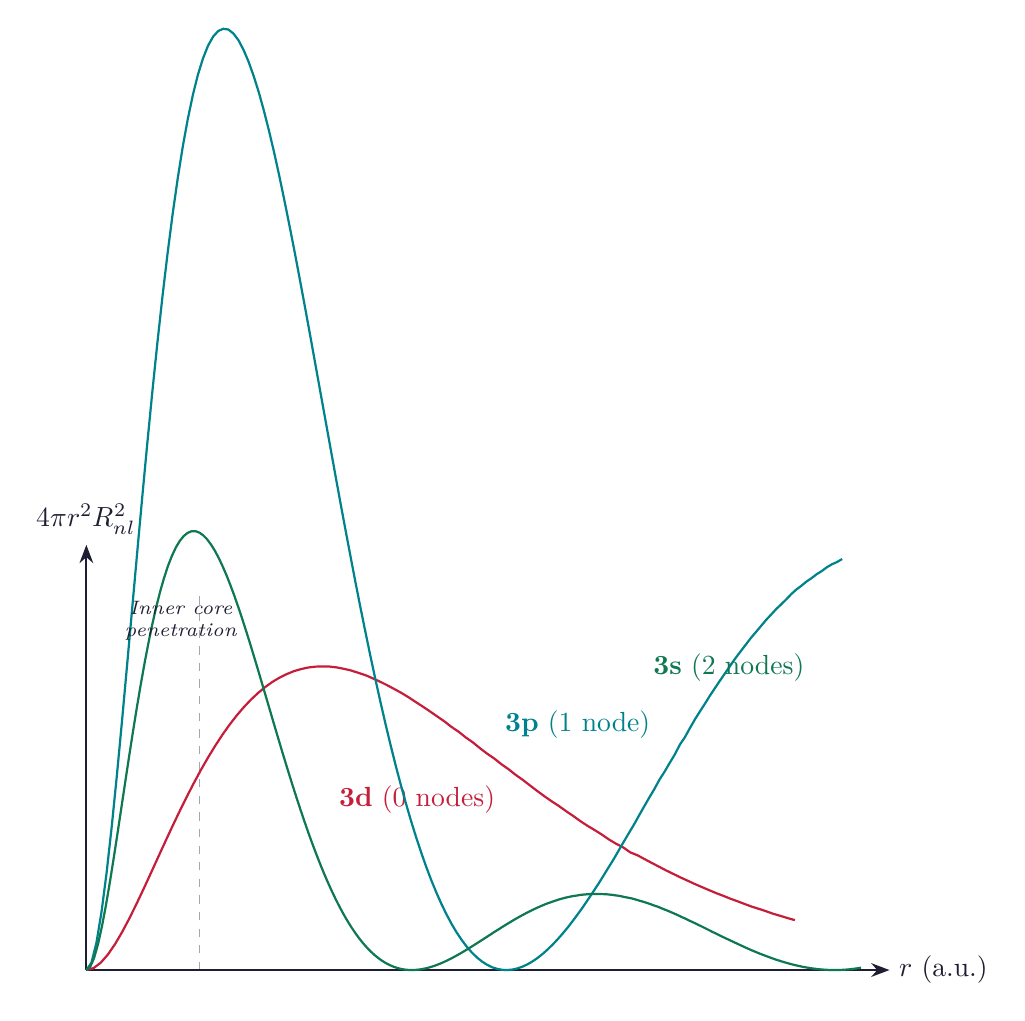
\begin{tikzpicture}[scale=1.2]
  % Draw axes
  \draw[arrow] (0,0) -- (8.5,0) node[right] {$r$ (a.u.)};
  \draw[arrow] (0,0) -- (0,4.5) node[above] {$4\pi r^2 R_{nl}^2$};
  
  % Plot 3d (1 peak, no nodes)
  \draw[thick, color=myred, domain=0:7.5, samples=100] 
    plot (\x, {3.8 * (\x)^2 * exp(-0.8*\x)});
  \node[color=myred] at (3.5, 1.8) {\textbf{3d} (0 nodes)};
  
  % Plot 3p (2 peaks, 1 node)
  \draw[thick, color=myteal, domain=0:8.0, samples=150] 
    plot (\x, {1.8 * (\x)^2 * (4 - 0.9*\x)^2 * exp(-0.7*\x)});
  \node[color=myteal] at (5.2, 2.6) {\textbf{3p} (1 node)};
  
  % Plot 3s (3 peaks, 2 nodes)
  \draw[thick, color=mygreen, domain=0:8.2, samples=200] 
    plot (\x, {0.6 * (\x)^2 * (6 - 2.5*\x + 0.22*(\x)^2)^2 * exp(-0.6*\x)});
  \node[color=mygreen] at (6.8, 3.2) {\textbf{3s} (2 nodes)};
  
  % Highlight penetration area close to nucleus
  \draw[dashed, color=mydark, opacity=0.4] (1.2, 0) -- (1.2, 4.0);
  \node[align=center, font=\scriptsize\itshape, color=mydark] at (1.0, 3.7) {Inner core\\penetration};
\end{tikzpicture}
\par\vspace{4pt}
\small\color{mydark}
Comparison of radial probability density distribution for $3s$, $3p$, and $3d$ orbitals. Note that while the main (outermost) peak of the $3d$ orbital is closer to the nucleus than that of $3s$, the $3s$ orbital has two inner peaks that penetrate the inner electron core, making $3s$ more stable (lower in energy).
\end{center}
\end{tcolorbox}

\subsection{Variations of Orbital Energies in the Periodic Table}
In hydrogenic atoms, the energy of an orbital depends solely on the principal quantum number $n$:
\[ E_n = -\frac{13.6 \cdot Z^2}{n^2}\ \text{eV} \]
Hence, $3s, 3p$, and $3d$ are degenerate (have the same energy).

In multi-electron atoms, the electrostatic shielding splits this degeneracy. The energy of an orbital depends on both $n$ and the azimuthal quantum number $l$. The ordering of orbital energies follows the $(n+l)$ rule (Madelung's rule):
\begin{enumerate}
  \item Orbitals are filled in order of increasing $(n+l)$ values.
  \item If two orbitals have the same $(n+l)$ value, the one with the lower $n$ value is filled first.
\end{enumerate}

Thus, for any shell $n$, the energy order is split by penetration and shielding into:
\[ E_{ns} < E_{np} < E_{nd} < E_{nf} \]

As the nuclear charge ($Z$) increases across the periodic table, the energies of all orbitals decrease (they become more stable) because the electrostatic attraction of the nucleus increases. However, they do not decrease at the same rate:
\begin{itemize}[leftmargin=*, itemsep=2pt]
  \item Inner shell orbitals drop rapidly in energy as $Z$ increases.
  \item Outer $s$ and $p$ orbitals drop steadily.
  \item $d$ and $f$ orbitals show a sudden, steep drop in energy (known as \textbf{orbital collapse}) when they begin to fill (e.g., $3d$ becomes lower in energy than $4s$ in transition metal cations).
\end{itemize}

\subsection{Electronic Configurations and Hund's Exchange Energy}
The ground-state electronic configuration of an atom is governed by three fundamental principles:
\begin{enumerate}
  \item \textbf{Aufbau Principle:} Electrons occupy the lowest energy orbitals available.
  \item \textbf{Pauli Exclusion Principle:} No two electrons in an atom can have the same set of four quantum numbers (an orbital can hold a maximum of 2 electrons with opposite spins).
  \item \textbf{Hund's Rule of Maximum Multiplicity:} For degenerate orbitals (orbitals with the same energy), the lowest energy configuration is the one that maximises the total spin multiplicity ($2S+1$). Electrons occupy degenerate orbitals singly with parallel spins before pairing begins.
\end{enumerate}

\textbf{Anomalous Electronic Configurations:}
Chromium ($Cr$, $Z=24$) and Copper ($Cu$, $Z=29$) are classic exceptions to the Aufbau rule:
\begin{itemize}[leftmargin=*, itemsep=1pt]
  \item Expected $Cr$: $[\text{Ar}]3d^4 4s^2$ \quad$\to$\quad Actual $Cr$: $[\text{Ar}]3d^5 4s^1$
  \item Expected $Cu$: $[\text{Ar}]3d^9 4s^2$ \quad$\to$\quad Actual $Cu$: $[\text{Ar}]3d^{10} 4s^1$
\end{itemize}

This anomalous behavior is driven by two main factors that stabilize half-filled ($d^5$) and fully-filled ($d^{10}$) subshells:
\begin{enumerate}
  \item \textbf{Symmetrical Distribution of Charge:} Symmetrical charge distribution around the nucleus reduces electron-electron repulsions and stabilizes the system.
  \item \textbf{Exchange Energy ($E_{\text{ex}}$):} Electrons with parallel spins in degenerate orbitals can exchange their positions. Each exchange releases a small quantum of energy called exchange energy, which stabilizes the atom. The number of possible exchanges ($P$) for $n$ parallel-spin electrons is given by:
  \begin{tcolorbox}[formulabox, title={Exchange Count Equation}]
    \[ P = \frac{n(n-1)}{2} \]
  \end{tcolorbox}
\end{enumerate}

\begin{tcolorbox}[examplebox, title={Example 2.1: Exchange Energy Comparison in Chromium ($Cr$)}]
  Compare the number of possible exchanges and stability between the expected and actual electronic configurations of Chromium ($Z=24$).
  \par\vspace{4pt}
  \textbf{Solution:}
  Let $K$ be the stabilizing exchange energy per exchange pair.
  \par\vspace{4pt}
  \textbf{Configuration A: $[\text{Ar}]3d^4 4s^2$ (Expected)}
  \begin{itemize}[leftmargin=*, itemsep=2pt]
    \item $3d^4$ subshell has 4 parallel-spin electrons ($\uparrow, \uparrow, \uparrow, \uparrow, \text{blank}$).
      \[ P_{3d} = \frac{4(4-1)}{2} = \frac{12}{2} = 6 \text{ exchanges} \]
    \item $4s^2$ has paired electrons ($\uparrow\downarrow$) which have opposite spins, so they cannot exchange.
    \item Total exchanges = $6$. Stabilization energy = $6K$.
  \end{itemize}
  \par\vspace{4pt}
  \textbf{Configuration B: $[\text{Ar}]3d^5 4s^1$ (Actual)}
  \begin{itemize}[leftmargin=*, itemsep=2pt]
    \item $3d^5$ subshell has 5 parallel-spin electrons ($\uparrow, \uparrow, \uparrow, \uparrow, \uparrow$).
      \[ P_{3d} = \frac{5(5-1)}{2} = \frac{20}{2} = 10 \text{ exchanges} \]
    \item $4s^1$ has 1 electron ($\uparrow$) which has a parallel spin to the $3d$ electrons. However, it resides in a different principal shell ($n=4$ vs $n=3$) and cannot exchange with $3d$.
    \item Total exchanges = $10$. Stabilization energy = $10K$.
  \end{itemize}
  \par\vspace{4pt}
  \textbf{Conclusion:} The actual configuration ($3d^5 4s^1$) has $10 - 6 = 4$ more exchanges than the expected configuration ($3d^4 4s^2$). The extra exchange energy ($4K$) easily overcomes the minor energy penalty of promoting an electron from $4s$ to $3d$, locking in the half-filled state.
\end{tcolorbox}

\begin{tcolorbox}[exambox, title={Exam Points: Penetration and Configurations}]
  \begin{itemize}[leftmargin=*, itemsep=2pt, topsep=2pt]
    \item \textbf{Penetration Order:} Always state the order $s > p > d > f$ and explain it using radial node count ($n-l-1$).
    \item \textbf{Energy splitting:} Explain why the $3s$ orbital is more stable than $3d$ in sodium despite having the same principal quantum number.
    \item \textbf{Exchange Energy:} Be ready to show the exchange energy calculation for $Cr$ or $Cu$ using the formula $P = \frac{n(n-1)}{2}$ to explain the stability of half/fully-filled shells.
    \item \textbf{Aufbau exceptions:} Clearly outline the configurations for $Cr$ ($3d^5 4s^1$) and $Cu$ ($3d^{10} 4s^1$).
  \end{itemize}
\end{tcolorbox}

% =============================================================================
\section{Atomic and Ionic Sizes}
% =============================================================================

\begin{tcolorbox}[defbox, title={Definitions: Types of Radii}]
  \textbf{Covalent Radius:} One-half of the distance between the nuclei of two identical atoms joined by a single covalent bond in a molecule (e.g., $d_{\text{Cl-Cl}} = 1.98\text{ \AA} \implies r_{\text{cov}} = 0.99\text{ \AA}$).
  \par\vspace{4pt}
  \textbf{Metallic (Crystal) Radius:} One-half of the internuclear distance between two adjacent metal cations in a metallic crystal lattice.
  \par\vspace{4pt}
  \textbf{Van der Waals Radius:} One-half of the closest internuclear distance between two non-bonded adjacent atoms belonging to two neighboring molecules in the solid state.
  \par\vspace{4pt}
  \textbf{Ionic Radius:} The effective distance from the center of the nucleus of an ion up to which it exerts influence on its electron cloud.
\end{tcolorbox}

\subsection{Comparison of Radii Types}
Because the van der Waals force is weak and non-binding, the nuclei of non-bonded adjacent atoms in a solid lattice remain relatively far apart. In contrast, covalent bonds involve significant overlap of valence electron clouds, drawing the nuclei close together. Metallic bonds represent an intermediate state where valence electrons are shared as a delocalized "sea." Therefore, for any given element, the relative sizes of these radii follow the order:

\begin{tcolorbox}[formulabox, title={Radii Comparison Trend}]
  \[ r_{\text{van der Waals}} > r_{\text{metallic}} > r_{\text{covalent}} \]
\end{tcolorbox}

\subsection{Periodic Trends in Atomic Sizes}
Atomic size is determined by the balance between the principal quantum number $n$ (which dictates the shell distance) and the effective nuclear charge $Z_{\text{eff}}$ (which pulls the shell closer).

\textbf{1. Across a Period (Left to Right):}
As we move across a period, $n$ remains constant while the effective nuclear charge $Z_{\text{eff}}$ increases by $\sim 0.65$ per element. The stronger electrostatic attraction pulls the electrons closer to the nucleus, causing the atomic radius to \textbf{decrease} steadily.

\textbf{2. Down a Group (Top to Bottom):}
As we move down a group, the principal quantum number $n$ increases (new energy shells are added). Although the nuclear charge increases, the shielding effect of the inner shells keeps $Z_{\text{eff}}$ relatively constant. The addition of new shells overrides the slight increases in $Z_{\text{eff}}$, causing the atomic radius to \textbf{increase} significantly.

\begin{tcolorbox}[tikzbox, title={Atomic Radii Trends Across Period 2 and Period 3}]
\begin{center}
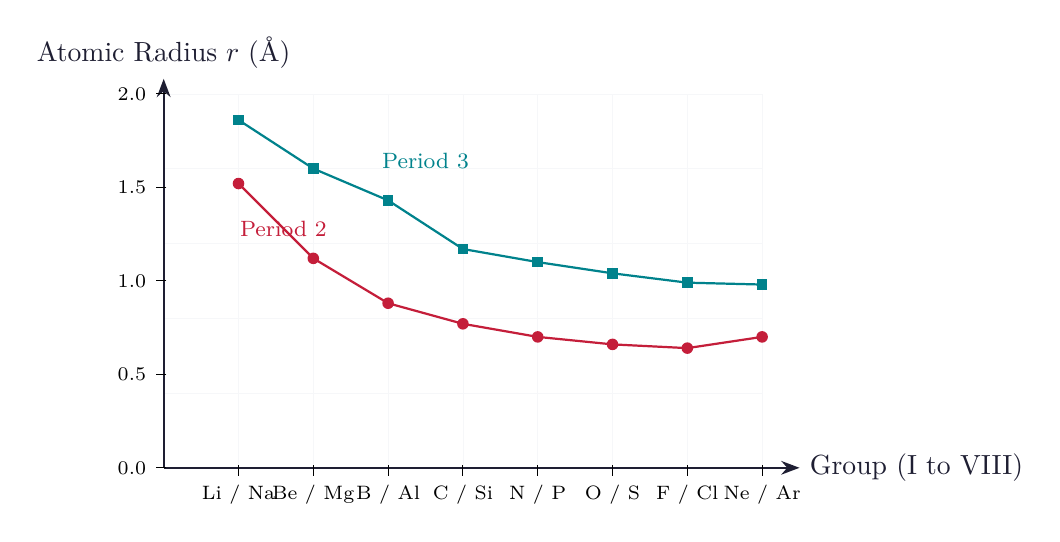
\begin{tikzpicture}[scale=0.95]
  % Draw Grid
  \draw[very thin, color=mygray, step=1.0] (0,0) grid (8,5);
  
  % Draw axes
  \draw[arrow] (0,0) -- (8.5,0) node[right] {Group (I to VIII)};
  \draw[arrow] (0,0) -- (0,5.2) node[above] {Atomic Radius $r$ (\text{\AA})};
  
  % Y-axis labels (0 to 2.0 A)
  \foreach \y/\label in {0/0.0, 1.25/0.5, 2.5/1.0, 3.75/1.5, 5.0/2.0} {
    \draw (1pt,\y) -- (-3pt,\y) node[left, font=\scriptsize] {\label};
  }
  
  % X-axis Group labels
  \foreach \x/\gp in {1/{Li / Na}, 2/{Be / Mg}, 3/{B / Al}, 4/{C / Si}, 5/{N / P}, 6/{O / S}, 7/{F / Cl}, 8/{Ne / Ar}} {
    \draw (\x,1pt) -- (\x,-3pt);
  }
  \node[below, font=\scriptsize] at (1, -0.1) {Li / Na};
  \node[below, font=\scriptsize] at (2, -0.1) {Be / Mg};
  \node[below, font=\scriptsize] at (3, -0.1) {B / Al};
  \node[below, font=\scriptsize] at (4, -0.1) {C / Si};
  \node[below, font=\scriptsize] at (5, -0.1) {N / P};
  \node[below, font=\scriptsize] at (6, -0.1) {O / S};
  \node[below, font=\scriptsize] at (7, -0.1) {F / Cl};
  \node[below, font=\scriptsize] at (8, -0.1) {Ne / Ar};

  % Period 2 Data: Li(1.52), Be(1.12), B(0.88), C(0.77), N(0.70), O(0.66), F(0.64), Ne(0.70)
  % Scaling: y_plot = y_val * 2.5
  \coordinate (P2_1) at (1, 3.8);  % Li
  \coordinate (P2_2) at (2, 2.8);  % Be
  \coordinate (P2_3) at (3, 2.2);  % B
  \coordinate (P2_4) at (4, 1.925); % C
  \coordinate (P2_5) at (5, 1.75); % N
  \coordinate (P2_6) at (6, 1.65); % O
  \coordinate (P2_7) at (7, 1.6);  % F
  \coordinate (P2_8) at (8, 1.75); % Ne (vdW)
  
  \draw[thick, color=myred] (P2_1) -- (P2_2) -- (P2_3) -- (P2_4) -- (P2_5) -- (P2_6) -- (P2_7) -- (P2_8);
  \foreach \i in {1,...,8} { \fill[color=myred] (P2_\i) circle (2.2pt); }
  \node[color=myred, font=\footnotesize] at (1.6, 3.2) {Period 2};

  % Period 3 Data: Na(1.86), Mg(1.60), Al(1.43), Si(1.17), P(1.10), S(1.04), Cl(0.99), Ar(0.98)
  % Scaling: y_plot = y_val * 2.5
  \coordinate (P3_1) at (1, 4.65); % Na
  \coordinate (P3_2) at (2, 4.0);  % Mg
  \coordinate (P3_3) at (3, 3.575);% Al
  \coordinate (P3_4) at (4, 2.925);% Si
  \coordinate (P3_5) at (5, 2.75); % P
  \coordinate (P3_6) at (6, 2.6);  % S
  \coordinate (P3_7) at (7, 2.475);% Cl
  \coordinate (P3_8) at (8, 2.45); % Ar (vdW)
  
  \draw[thick, color=myteal] (P3_1) -- (P3_2) -- (P3_3) -- (P3_4) -- (P3_5) -- (P3_6) -- (P3_7) -- (P3_8);
  \foreach \i in {1,...,8} { \fill[color=myteal] (P3_\i) +(-2pt,-2pt) rectangle +(2pt,2pt); }
  \node[color=myteal, font=\footnotesize] at (3.5, 4.1) {Period 3};

\end{tikzpicture}
\par\vspace{4pt}
\small\color{mydark}
Periodic atomic radii trends. Covalent radii decrease across Period 2 and 3. The noble gases (Ne, Ar) exhibit larger values than halogens because their radii are measured as non-bonding van der Waals radii, which do not involve orbital overlap.
\end{center}
\end{tcolorbox}

\subsection{Ionic Radii and Coordination Number Dependency}
Ionic radii depend heavily on the electric charge and configuration of the ion:
\begin{itemize}[leftmargin=*, itemsep=2pt]
  \item \textbf{Cations are always smaller than parent atoms:} Loss of valence electrons reduces electron-electron repulsion, allowing the remaining electrons to be pulled closer by the same nuclear charge (e.g., $r_{\text{Na}} = 1.86\text{ \AA}$ vs $r_{\text{Na}^+} = 1.02\text{ \AA}$).
  \item \textbf{Anions are always larger than parent atoms:} Gaining valence electrons increases electron-electron repulsions, expanding the electron cloud without any increase in nuclear charge (e.g., $r_{\text{Cl}} = 0.99\text{ \AA}$ vs $r_{\text{Cl}^-} = 1.81\text{ \AA}$).
\end{itemize}

\textbf{Coordination Number (CN) Dependency:}
An ion's radius is not a fixed constant. It varies with its coordination environment. As the coordination number (number of nearest neighbors) increases, the electrostatic repulsions between the surrounding ligands/ions squeeze the central ion less, or rather, the central ion must expand its coordination sphere to accommodate more ligands. Therefore, \textbf{ionic radius increases as the coordination number increases}. For example, the ionic radius of $\text{Li}^+$ increases from $0.59\text{ \AA}$ (for $\text{CN} = 4$) to $0.76\text{ \AA}$ (for $\text{CN} = 6$).

\subsection{Isoelectronic Series}
An isoelectronic series consists of atoms/ions that possess the same number of electrons but different nuclear charges ($Z$). 

For an isoelectronic series, the shielding constant $\sigma$ is essentially constant because the number and distribution of electrons are identical. Therefore, the effective nuclear charge experienced by the electrons is determined purely by the atomic number ($Z$). As $Z$ increases, the nuclear attraction pulls the same number of electrons closer. Thus, \textbf{in an isoelectronic series, size decreases as the atomic number ($Z$) increases}.

\begin{tcolorbox}[examplebox, title={Example 3.1: Isoelectronic Series Comparison}]
  Arrange the following species in order of decreasing size: $\text{O}^{2-}$, $\text{F}^-$, $\text{Na}^+$, $\text{Mg}^{2+}$, $\text{Al}^{3+}$.
  \par\vspace{4pt}
  \textbf{Solution:}
  All five species have exactly 10 electrons ($1s^2 2s^2 2p^6$) and are isoelectronic. We compile their nuclear charges ($Z$):
  \begin{center}
  \begin{tabularx}{0.8\linewidth}{|B{3cm}|Y|Y|Y|Y|Y|}
    \hline
    \textbf{Species} & $\text{O}^{2-}$ & $\text{F}^-$ & $\text{Na}^+$ & $\text{Mg}^{2+}$ & $\text{Al}^{3+}$ \\
    \hline
    \textbf{Nuclear Charge ($Z$)} & 8 & 9 & 11 & 12 & 13 \\
    \hline
    \textbf{Ionic Radius (\text{\AA})} & 1.40 & 1.33 & 1.02 & 0.72 & 0.54 \\
    \hline
  \end{tabularx}
  \end{center}
  As $Z$ increases from 8 to 13, the positive charge of the nucleus increases, pulling the 10 electrons tighter.
  \par\vspace{4pt}
  Therefore, the order of decreasing size is:
  \[ \text{O}^{2-} > \text{F}^- > \text{Na}^+ > \text{Mg}^{2+} > \text{Al}^{3+} \]
\end{tcolorbox}

\subsection{Lanthanide Contraction and Its Consequences}
The \textbf{Lanthanide Contraction} refers to the steady, progressive decrease in the atomic and ionic radii of the lanthanide elements (from Lanthanum ($Z=57$) to Lutetium ($Z=71$)) as the atomic number increases.

\textbf{Cause:}
As we move along the lanthanide series, electrons are added successively to the inner $4f$ subshell. The $4f$ orbitals are highly diffuse in space. As a result, the shielding of one $4f$ electron by another is extremely poor ($\sigma \approx 0.35$). However, with each element, the nuclear charge $Z$ increases by $+1$. Because the $4f$ electrons fail to screen the increasing positive charge, the effective nuclear charge felt by all outer electrons increases steadily. This pulls the outer shell closer, causing a steady contraction.

\textbf{Critical Consequences of Lanthanide Contraction:}
\begin{enumerate}
  \item \textbf{Size Similarity of $4d$ and $5d$ Elements:} In transition metal groups, we normally expect a significant increase in atomic size from the 2nd transition series ($4d$) to the 3rd transition series ($5d$) due to the addition of a new principal shell. However, the lanthanide contraction (which occurs between the $4d$ and $5d$ series) cancels out this expected increase.
    \par
    Consequently, elements of the 2nd and 3rd transition series in the same group have almost identical atomic and ionic radii.
    \begin{itemize}
      \item Group 4: $\text{Zr}$ ($4d$, $r \approx 1.60\text{ \AA}$) and $\text{Hf}$ ($5d$, $r \approx 1.59\text{ \AA}$).
      \item Group 5: $\text{Nb}$ ($4d$, $r \approx 1.46\text{ \AA}$) and $\text{Ta}$ ($5d$, $r \approx 1.46\text{ \AA}$).
    \end{itemize}
    This structural similarity makes their chemical separation extremely difficult.
  \item \textbf{Extreme Densities of Post-Lanthanide Metals:} Because the $5d$ transition elements have nearly identical sizes to their $4d$ counterparts but possess much higher atomic masses (due to 32 additional protons and neutrons), their densities are roughly double. For example, the density of Iridium ($22.56\ \text{g\,cm}^{-3}$) is twice that of Rhodium ($12.41\ \text{g\,cm}^{-3}$).
\end{enumerate}

\begin{tcolorbox}[exambox, title={Exam Points: Atomic and Ionic Sizes}]
  \begin{itemize}[leftmargin=*, itemsep=2pt, topsep=2pt]
    \item \textbf{Radii Comparison:} Explain why $r_{\text{vdW}} > r_{\text{met}} > r_{\text{cov}}$ using orbital overlap argument.
    \item \textbf{Isoelectronic Series:} Be prepared to write ionic size orders and explain them by referencing the nuclear charge ($Z$).
    \item \textbf{Lanthanide Contraction Cause:} State clearly that the cause is the "poor shielding of diffuse $4f$ orbitals."
    \item \textbf{Zr/Hf pair:} This is a MAKAUT favorite. Explain why Zr and Hf have identical properties by referencing the Lanthanide Contraction.
  \end{itemize}
\end{tcolorbox}

% =============================================================================
\section{Ionization Energy \& Electron Affinity}
% =============================================================================

\begin{tcolorbox}[defbox, title={Definitions: Ionization Energy and Electron Affinity}]
  \textbf{Ionization Energy (IE):} The minimum energy required to remove the most loosely bound electron from an isolated gaseous atom in its ground state:
  \[ \text{M(g)} + \text{IE} \to \text{M}^+\text{(g)} + e^- \]
  \par\vspace{4pt}
  \textbf{Electron Affinity (EA):} The amount of energy released when an electron is added to an isolated neutral gaseous atom to form a univalent anion:
  \[ \text{X(g)} + e^- \to \text{X}^-\text{(g)} + \text{EA} \]
  Its thermodynamic counterpart is \textbf{Electron Gain Enthalpy} ($\Delta_{\text{eg}}H \approx -\text{EA}$).
\end{tcolorbox}

\subsection{Successive Ionization Energies}
Removing successive electrons from an atom requires progressively larger amounts of energy. For any element, the successive ionization energies follow the order:
\[ IE_1 < IE_2 < IE_3 < IE_4 \dots \]

This trend is caused by:
\begin{enumerate}
  \item \textbf{Electrostatic Charge:} Removing an electron from a neutral atom ($IE_1$) only requires overcoming neutral forces. However, removing an electron from a positively charged cation ($IE_2$, $IE_3$) requires pulling a negative electron away from an increasingly positive net charge.
  \item \textbf{Size Contraction:} With each electron lost, electron-electron repulsion decreases, allowing the remaining orbital cloud to contract closer to the nucleus. This stronger binding increases the energy required for further ionization.
\end{enumerate}

A sudden, dramatic jump in successive ionization energies (e.g., $IE_2 \gg IE_1$ for Sodium) signifies the transition from removing valence-shell electrons to removing core-shell electrons from a highly stable noble-gas configuration.

\subsection{Factors Affecting Ionization Energy}
The ionization energy of an atom is determined by:
\begin{itemize}[leftmargin=*, itemsep=2pt]
  \item \textbf{Atomic Size:} As size increases, valence electrons are farther from the nucleus, experience less attraction, and are easier to remove ($\text{IE} \propto 1/r$).
  \item \textbf{Effective Nuclear Charge ($Z_{\text{eff}}$):} A higher $Z_{\text{eff}}$ pulls valence electrons tighter, increasing the energy needed to remove them ($\text{IE} \propto Z_{\text{eff}}$).
  \item \textbf{Penetration Effect:} Orbitals penetrate the inner electron core in the order $s > p > d > f$. An $s$ electron resides closer to the nucleus and experiences less shielding than a $p$ electron of the same shell, making it harder to ionize.
  \item \textbf{Electronic Configuration:} Half-filled ($d^5, p^3$) and fully-filled ($d^{10}, s^2$) subshells have extra stability due to exchange energy and symmetric charge distribution. Removing an electron from these stable configurations requires higher energy.
\end{itemize}

\subsection{Anomalies in Periodic IE Trends}
Across a period, ionization energy generally increases due to the steady increase in $Z_{\text{eff}}$. However, there are two distinct anomalies in every period:

\begin{tcolorbox}[examplebox, title={Anomaly 1: Beryllium ($Z=4$) vs. Boron ($Z=5$)}]
  Explain why the first ionization energy of Beryllium is higher than that of Boron ($IE_1(\text{Be}) = 899\ \text{kJ\,mol}^{-1}$ vs $IE_1(\text{B}) = 801\ \text{kJ\,mol}^{-1}$).
  \par\vspace{4pt}
  \textbf{Solution:}
  Let us inspect their ground-state configurations:
  \begin{itemize}[leftmargin=1cm, itemsep=2pt]
    \item $\text{Be}$: $1s^2 2s^2$ (fully-filled $2s$ subshell).
    \item $\text{B}$: $1s^2 2s^2 2p^1$ (partially-filled $2p$ subshell).
  \end{itemize}
  Two factors favor higher ionization energy for Beryllium:
  \begin{enumerate}
    \item \textbf{Penetration:} The electron to be removed from Beryllium resides in a $2s$ orbital, whereas the electron to be removed from Boron resides in a $2p$ orbital. Because $2s$ penetrates the inner core closer to the nucleus than $2p$, the $2s$ electron is bound more tightly.
    \item \textbf{Subshell Stability:} The $2s^2$ configuration of Beryllium is a fully-filled, closed-shell state which possesses extra electrostatic stability. Removing an electron disrupts this stable subshell.
  \end{enumerate}
  Therefore, Beryllium has a higher first ionization energy than Boron.
\end{tcolorbox}

\begin{tcolorbox}[examplebox, title={Anomaly 2: Nitrogen ($Z=7$) vs. Oxygen ($Z=8$)}]
  Explain why the first ionization energy of Nitrogen is higher than that of Oxygen ($IE_1(\text{N}) = 1402\ \text{kJ\,mol}^{-1}$ vs $IE_1(\text{O}) = 1314\ \text{kJ\,mol}^{-1}$).
  \par\vspace{4pt}
  \textbf{Solution:}
  Let us inspect their valence configurations:
  \begin{itemize}[leftmargin=1cm, itemsep=2pt]
    \item $\text{N}$: $2s^2 2p^3$ (half-filled $2p$ subshell: $2p_x^1 2p_y^1 2p_z^1$).
    \item $\text{O}$: $2s^2 2p^4$ (partially-filled $2p$ subshell: $2p_x^2 2p_y^1 2p_z^1$).
  \end{itemize}
  \begin{enumerate}
    \item \textbf{Exchange Energy:} Nitrogen has a stable, half-filled $2p^3$ configuration with 3 parallel-spin electrons. This configuration is stabilized by maximum exchange energy ($3$ exchange pairs) and symmetrical charge distribution.
    \item \textbf{Inter-electronic Repulsion:} In Oxygen's $2p^4$ configuration, one of the $2p$ orbitals ($2p_x$) contains a pair of electrons. These two electrons sharing the same orbital volume experience significant electrostatic repulsion. Removing one of these electrons relieves this repulsion and yields the highly stable half-filled $2p^3$ configuration.
  \end{enumerate}
  Consequently, it is easier to remove an electron from Oxygen than from Nitrogen, resulting in $IE_1(\text{N}) > IE_1(\text{O})$.
\end{tcolorbox}

\subsection{Electron Affinity and Successive Values}
Electron affinity (EA) measures the energy released when a gaseous atom gains an electron. If the process is exothermic, $\Delta_{\text{eg}}H$ is negative and EA is positive.

\textbf{Successive Electron Affinities:}
While the first electron affinity ($EA_1$) of most elements (like halogens, chalcogens) is positive (exothermic), the second electron affinity ($EA_2$) is \textbf{always highly negative (endothermic)}.
\par
For example, adding the first electron to Oxygen is exothermic:
\[ \text{O(g)} + e^- \to \text{O}^-\text{(g)} \quad \Delta_{\text{eg}}H_1 = -141\ \text{kJ\,mol}^{-1} \quad (EA_1 = +141\ \text{kJ\,mol}^{-1}) \]
However, adding the second electron to form oxide ($\text{O}^{2-}$) is highly endothermic:
\[ \text{O}^-\text{(g)} + e^- \to \text{O}^{2-}\text{(g)} \quad \Delta_{\text{eg}}H_2 = +780\ \text{kJ\,mol}^{-1} \quad (EA_2 = -780\ \text{kJ\,mol}^{-1}) \]
This occurs because the incoming electron experiences intense electrostatic repulsion from the existing negative charge of the $\text{O}^-$ anion. Overcoming this repulsion requires a significant input of energy. The formation of stable oxide lattices (like $\text{MgO}$ or $\text{Na}_2\text{O}$) in the solid state is driven by the very high lattice energy of the resulting ionic crystal, which easily compensates for this endothermic step.

\subsection{Anomalies in Electron Affinity Trends}
Within a group, electron affinity generally decreases down the column as atomic size increases, because the incoming electron is added farther from the nucleus. However, the elements of the \textbf{second period} (specifically F, O, N) exhibit anomalously low electron affinities compared to the elements of the \textbf{third period} (Cl, S, P):

\begin{tcolorbox}[examplebox, title={Anomaly: Fluorine vs. Chlorine Electron Affinity}]
  Explain why Chlorine has a higher electron affinity than Fluorine ($EA(\text{Cl}) = 349\ \text{kJ\,mol}^{-1}$ vs $EA(\text{F}) = 328\ \text{kJ\,mol}^{-1}$), even though Fluorine is smaller and more electronegative.
  \par\vspace{4pt}
  \textbf{Solution:}
  \begin{enumerate}
    \item \textbf{Valence Shell Volume:} Fluorine resides in the second period ($n=2$), and its valence electrons occupy a very compact $2p$ subshell. Chlorine resides in the third period ($n=3$), and its valence electrons occupy a much larger, more diffuse $3p$ subshell.
    \item \textbf{Inter-electronic Repulsion:} When an electron is added to the compact $2p$ subshell of Fluorine, the incoming electron experiences intense electrostatic repulsion from the seven electrons already packed in that small volume. This repulsion offsets some of the energy released by nuclear attraction.
    \item In Chlorine, the larger volume of the $3p$ subshell distributes the electron density over a wider area. The inter-electronic repulsion felt by the incoming electron is significantly lower.
  \end{enumerate}
  Therefore, more net energy is released when Chlorine gains an electron, resulting in $EA(\text{Cl}) > EA(\text{F})$.
\end{tcolorbox}

\subsection{Comparison Table: Ionization Energy vs. Electron Affinity}
\par\noindent
\begin{tabularx}{\linewidth}{|B{4.5cm}|Y|Y|}
\hline
\textbf{Property} & \textbf{Ionization Energy (IE)} & \textbf{Electron Affinity (EA)} \\
\hline
\textbf{Process} & Removal of an electron ($\text{M} \to \text{M}^+ + e^-$). & Addition of an electron ($\text{X} + e^- \to \text{X}^-$). \\
\hline
\textbf{Energy Change} & Always endothermic ($\Delta H > 0$, energy absorbed). & Usually exothermic for $EA_1$ ($\Delta H < 0$, energy released). Always endothermic for $EA_2$. \\
\hline
\textbf{Noble Gas Values} & Exceptionally high (stable closed-shell configurations). & Extremely low or negative (energy must be forced in to open a new shell). \\
\hline
\textbf{General Periodic Trend} & Increases across a period, decreases down a group. & Becomes more positive (exothermic) across a period, decreases down a group. \\
\hline
\textbf{Key Group 17 Anomaly} & $\text{IE}(\text{F}) > \text{IE}(\text{Cl})$ (normal size trend). & $\text{EA}(\text{Cl}) > \text{EA}(\text{F})$ (repulsion anomaly). \\
\hline
\end{tabularx}
\vspace{6pt}

\begin{tcolorbox}[exambox, title={Exam Points: IE and EA}]
  \begin{itemize}[leftmargin=*, itemsep=2pt, topsep=2pt]
    \item \textbf{Anomalous pairs:} Always explain Be/B and N/O in exams by writing down the subshell configurations.
    \item \textbf{F/Cl EA comparison:} This is the most common EA question. Focus on "charge density" and "inter-electronic repulsion in the compact $2p$ subshell of F."
    \item \textbf{Successive EA:} Explain why $EA_2$ is always negative (endothermic) by referencing the repulsion from the mono-negative anion.
    \item \textbf{IE Successive Trends:} Be ready to explain the massive jump in successive ionization energies (e.g. $IE_1$ vs $IE_2$ for alkali metals) as core-shell disruption.
  \end{itemize}
\end{tcolorbox}

% =============================================================================
\section{Electronegativity \& Polarizability}
% =============================================================================

\begin{tcolorbox}[defbox, title={Definitions: Electronegativity and Polarizability}]
  \textbf{Electronegativity ($\chi$):} The relative tendency of an atom in a molecule to attract the shared pair of electrons towards itself.
  \par\vspace{4pt}
  \textbf{Polarizing Power:} The ability of a cation to distort the electron cloud of an adjacent anion.
  \par\vspace{4pt}
  \textbf{Polarizability:} The ease with which the electron cloud of an anion can be distorted by a neighboring cation.
\end{tcolorbox}

\subsection{Electronegativity Scales}
Unlike ionization energy or electron affinity, electronegativity is not a direct thermodynamic property of an isolated atom. It represents a behavior within a bond, so it must be calculated using comparative scales:

\textbf{1. Pauling Scale (Bond Dissociation Energy Basis):}
Linus Pauling proposed that the excess bond energy of a polar bond $A-B$ over the average of pure homonuclear covalent bonds $A-A$ and $B-B$ is due to ionic-covalent resonance stabilization. The electronegativity difference is defined as:
\begin{tcolorbox}[formulabox, title={Pauling Electronegativity Difference}]
  \[ \chi_A - \chi_B = 0.102 \sqrt{\Delta} \]
  Where:
  \[ \Delta = E_{AB} - \sqrt{E_{AA} \cdot E_{BB}} \quad (\text{in kJ\,mol}^{-1}) \]
\end{tcolorbox}
Here, $\Delta$ represents the ionic resonance energy. Pauling arbitrarily assigned a value of $2.20$ to Hydrogen as an anchor to calibrate all other elements (Fluorine has the maximum value at $3.98$).

\textbf{2. Mulliken Scale (Atomic Energy Basis):}
Robert Mulliken proposed that an atom's ability to attract electrons in a bond is the average of its ionization energy (IE) and electron affinity (EA). If both values are measured in electron-volts ($\text{eV}$):
\begin{tcolorbox}[formulabox, title={Mulliken Electronegativity Equation}]
  \[ \chi_{\text{M}} = \frac{\text{IE} + \text{EA}}{2} \]
  To align Mulliken values with the Pauling scale:
  \[ \chi_{\text{P}} \approx \frac{\chi_{\text{M}}}{2.8} = \frac{\text{IE(eV)} + \text{EA(eV)}}{5.6} \]
\end{tcolorbox}
If IE and EA are in $\text{kJ\,mol}^{-1}$, the denominator is $540$.

\textbf{3. Allred-Rochow Scale (Electrostatic Force Basis):}
A. L. Allred and E. G. Rochow defined electronegativity as the electrostatic force of attraction exerted by the effective nuclear charge ($Z_{\text{eff}}$) of the atom on a valence electron at its bonding radius.
\begin{tcolorbox}[formulabox, title={Allred-Rochow Electronegativity Equation}]
  \[ \chi_{\text{AR}} = 0.359 \frac{Z_{\text{eff}}}{r^2} + 0.744 \]
  Where:
  \begin{itemize}[leftmargin=1.5cm, itemsep=1pt]
    \item[$Z_{\text{eff}}$] = Effective nuclear charge calculated using Slater's rules.
    \item[$r$] = Covalent radius of the atom (in \text{\AA}).
  \end{itemize}
\end{tcolorbox}

\begin{tcolorbox}[examplebox, title={Example 5.1: Calculation of Allred-Rochow Electronegativity for Carbon}]
  Calculate the Allred-Rochow electronegativity of Carbon given its covalent radius $r = 0.77\text{ \AA}$ and atomic number $Z = 6$.
  \par\vspace{4pt}
  \textbf{Solution:}
  \begin{enumerate}
    \item Calculate $Z_{\text{eff}}$ for a valence electron in Carbon using Slater's rules (from Example 1.1):
      \[ Z_{\text{eff}} = 3.25 \]
    \item Substitute $Z_{\text{eff}}$ and $r$ into the Allred-Rochow formula:
      \[ \chi_{\text{AR}} = 0.359 \left( \frac{3.25}{(0.77)^2} \right) + 0.744 \]
      \[ \chi_{\text{AR}} = 0.359 \left( \frac{3.25}{0.5929} \right) + 0.744 \approx 0.359 (5.48) + 0.744 \]
      \[ \chi_{\text{AR}} \approx 1.967 + 0.744 = 2.71 \]
  \end{enumerate}
  This calculated value ($2.71$) is very close to Carbon's experimental Pauling electronegativity ($2.55$).
\end{tcolorbox}

\subsection{Bond Character and the Hannay-Smith Equation}
The electronegativity difference between two bonded atoms determines the degree of polar covalent vs. ionic character in that bond. If $\Delta\chi = 0$, the bond is purely covalent. If $\Delta\chi > 1.7$, the bond is considered predominantly ionic.
\par
To calculate the percentage ionic character of a polar covalent bond, the \textbf{Hannay-Smith Equation} is used:

\begin{tcolorbox}[formulabox, title={Hannay-Smith Equation}]
  \[ \% \text{ Ionic Character} = 16 |\chi_A - \chi_B| + 3.5 |\chi_A - \chi_B|^2 \]
  Where $\chi_A$ and $\chi_B$ are the electronegativity values of the two bonded atoms.
\end{tcolorbox}

\begin{tcolorbox}[examplebox, title={Example 5.2: Calculating Ionic Character of Hydrogen Fluoride ($\text{HF}$)}]
  Calculate the percentage ionic character of the $\text{H-F}$ bond in hydrogen fluoride, given $\chi_{\text{F}} = 3.98$ and $\chi_{\text{H}} = 2.20$.
  \par\vspace{4pt}
  \textbf{Solution:}
  \begin{enumerate}
    \item Find the difference in electronegativity:
      \[ \Delta\chi = |\chi_{\text{F}} - \chi_{\text{H}}| = 3.98 - 2.20 = 1.78 \]
    \item Apply the Hannay-Smith equation:
      \[ \% \text{ Ionic Character} = 16 (1.78) + 3.5 (1.78)^2 \]
      \[ \% \text{ Ionic Character} = 28.48 + 3.5 (3.1684) \]
      \[ \% \text{ Ionic Character} = 28.48 + 11.09 = 39.57\% \]
  \end{enumerate}
  Thus, the bond in gaseous $\text{HF}$ is approximately $39.6\%$ ionic and $60.4\%$ covalent.
\end{tcolorbox}

\subsection{Polarizability and Fajans' Rules}
In an ideal ionic bond, electrons are completely transferred, producing spherical ions. However, in reality, when a small cation approaches a large anion, the positive charge of the cation attracts the outer electron cloud of the anion while repelling its nucleus. This distorts the anion's electron cloud, shifting electron density into the internuclear region, introducing covalent character into the ionic bond.

To predict the extent of this polarization (and thus the degree of covalent character), we use \textbf{Fajans' Rules}:

\begin{enumerate}
  \item \textbf{Small Cation Size:} A smaller cation has a higher charge density (charge-to-size ratio, $q/r$). It exerts a stronger electrostatic pull on the anion's electron cloud, increasing its polarizing power and covalent character (e.g., $\text{LiCl}$ is more covalent and soluble in organic solvents than $\text{KCl}$).
  \item \textbf{Large Anion Size:} In a large anion, the valence electrons are far from the nucleus and are shielded effectively by inner shells. The nucleus holds these electrons weakly, making the electron cloud soft and highly polarizable (e.g., $\text{LiI}$ is much more covalent than $\text{LiF}$).
  \item \textbf{High Ionic Charges:} High charges on either the cation or the anion increase the electrostatic attraction, driving stronger polarization and covalent character (e.g., $\text{AlCl}_3$ is covalent with a low melting point, whereas $\text{MgCl}_2$ and $\text{NaCl}$ are ionic).
  \item \textbf{Pseudo-Noble Gas Configuration of Cation ($ns^2 np^6 nd^{10}$):} Cations with a pseudo-noble gas configuration have greater polarizing power than those with a noble gas configuration ($ns^2 np^6$) of similar size and charge. This occurs because the $d$-electrons shield the nucleus poorly, allowing the cation to exert a stronger effective nuclear charge on the adjacent anion.
\end{enumerate}

\begin{tcolorbox}[examplebox, title={Example 5.3: Fajans' Rules Application}]
  Explain why Cuprous chloride ($\text{CuCl}$) is covalent and insoluble in water, whereas Sodium chloride ($\text{NaCl}$) is ionic and highly soluble, even though $\text{Cu}^+$ ($r = 0.96\text{ \AA}$) and $\text{Na}^+$ ($r = 0.95\text{ \AA}$) have nearly identical ionic sizes and identical charges.
  \par\vspace{4pt}
  \textbf{Solution:}
  Let us inspect the electronic configurations of the cations:
  \begin{itemize}[leftmargin=1cm, itemsep=2pt]
    \item $\text{Na}^+$: $1s^2 2s^2 2p^6$ (noble gas configuration, $8$-electron valence shell).
    \item $\text{Cu}^+$: $1s^2 2s^2 2p^6 3s^2 3p^6 3d^{10}$ (pseudo-noble gas configuration, $18$-electron valence shell).
  \end{itemize}
  The 10 electrons in the $3d$ subshell of $\text{Cu}^+$ are highly diffuse and shield the nuclear charge very poorly compared to the $s$ and $p$ electrons of $\text{Na}^+$. Consequently, $\text{Cu}^+$ has a much higher effective nuclear charge at its boundary. This allows it to polarize the electron cloud of the chloride ion ($\text{Cl}^-$) far more strongly than $\text{Na}^+$ can. This intense polarization introduces significant covalent character into $\text{CuCl}$, making it insoluble in polar water.
\end{tcolorbox}

\begin{tcolorbox}[exambox, title={Exam Points: Electronegativity and Fajans' Rules}]
  \begin{itemize}[leftmargin=*, itemsep=2pt, topsep=2pt]
    \item \textbf{Hannay-Smith Equation:} Memorize this equation ($16\Delta\chi + 3.5\Delta\chi^2$) for percentage ionic character calculations. It is a common numerical topic.
    \item \textbf{Allred-Rochow Scale:} Explain how it differs from Pauling and Mulliken scales by focusing on its physical basis (electrostatic force).
    \item \textbf{Fajans' Rules application:} Be prepared to explain melting point trends (e.g., why $\text{SnCl}_4$ is a liquid while $\text{SnCl}_2$ is a solid) or solubility trends using polarization.
    \item \textbf{Pseudo-noble gas configuration:} State clearly that $d$-electrons shield poorly, leading to higher polarizing power for cations like $\text{Cu}^+$, $\text{Ag}^+$, or $\text{Zn}^{2+}$.
  \end{itemize}
\end{tcolorbox}

% =============================================================================
\section{Oxidation States \& Coordination Numbers}
% =============================================================================

\begin{tcolorbox}[defbox, title={Definitions: Oxidation States, Coordination Numbers, and Geometries}]
  \textbf{Oxidation State (OS):} The formal charge assigned to an atom in a chemical species, assuming all bonding electron pairs are completely transferred to the more electronegative partner.
  \par\vspace{4pt}
  \textbf{Coordination Number (CN):} The number of donor atoms directly bonded (via coordinate or covalent bonds) to the central metal atom or ion in a coordination complex.
  \par\vspace{4pt}
  \textbf{Coordination Geometry:} The specific spatial arrangement of the ligand donor atoms around the central metal atom or ion.
\end{tcolorbox}

\subsection{Variable Oxidation States in Transition Metals}
One of the most defining characteristics of transition metals ($d$-block elements) is their ability to exhibit multiple, variable oxidation states. For instance, Manganese ($Mn$) shows all oxidation states from $+2$ to $+7$.

This behavior is caused by:
\begin{enumerate}
  \item \textbf{Orbital Energy Proximity:} The energy difference between the outer $ns$ orbital and the inner $(n-1)d$ orbital is extremely small.
  \item \textbf{Bond Participation:} Because of this energy proximity, transition metals can lose or share not only their valence $ns$ electrons but also their $(n-1)d$ electrons when forming chemical bonds.
\end{enumerate}

\textbf{Stability Trends in Transition Metal Oxidation States:}
\begin{itemize}[leftmargin=*, itemsep=2pt]
  \item \textbf{Valence Core Stability ($d^0$, $d^5$, $d^{10}$):} Oxidation states that leave the metal ion with a stable half-filled ($d^5$) or fully-filled ($d^{10}$) subshell, or a completely empty ($d^0$) noble-gas core, are particularly stable.
    \begin{itemize}
      \item $\text{Sc}^{3+}$ ($3d^0$, stable noble-gas $[\text{Ar}]$ configuration).
      \item $\text{Fe}^{3+}$ ($3d^5$, stable half-filled configuration) is more stable and harder to oxidize than $\text{Fe}^{2+}$ ($3d^6$).
      \item $\text{Zn}^{2+}$ ($3d^{10}$, stable fully-filled configuration).
    \end{itemize}
  \item \textbf{High vs. Low States:} The highest oxidation state shown by a transition metal in the first series ($3d$) corresponds to the loss of all $4s$ and $3d$ electrons (e.g., $+7$ for $\text{Mn}$, $+6$ for $\text{Cr}$). Beyond Manganese ($Z=25$), the $3d$ orbitals become steadily lower in energy and more core-like, so high oxidation states become unstable and transition metals favor lower oxidation states ($+2$, $+3$).
\end{itemize}

\subsection{The Inert Pair Effect in Heavier \texorpdfstring{$p$}{p}-Block Elements}
In the main group elements ($s$- and $p$-block), elements generally exhibit an oxidation state corresponding to their group number (e.g., $+3$ for Group 13, $+4$ for Group 14). However, for the heavier elements in these groups (specifically those in Period 6: Thallium, Lead, Bismuth), the most stable oxidation state is \textbf{two units lower} than the group oxidation state.

This phenomenon is called the \textbf{Inert Pair Effect}, which refers to the reluctance of the outermost $s$-orbital electron pair ($ns^2$) to participate in chemical bonding:

\begin{tcolorbox}[defbox, title={Stable Oxidation States due to Inert Pair Effect}]
  \begin{itemize}[leftmargin=*, itemsep=4pt]
    \item \textbf{Group 13 ($\text{Al}, \text{Ga}, \text{In}, \text{Tl}$):} Stable OS for $\text{Al}$ is $+3$, but for $\text{Tl}$, it is $+1$ ($\text{Tl}^+$ is stable, $\text{Tl}^{3+}$ is a powerful oxidizing agent).
    \item \textbf{Group 14 ($\text{Si}, \text{Ge}, \text{Sn}, \text{Pb}$):} Stable OS for $\text{Si}, \text{Sn}$ is $+4$, but for $\text{Pb}$, it is $+2$ ($\text{Pb}^{2+}$ is stable, $\text{Pb}^{4+}$ is a powerful oxidizing agent).
    \item \textbf{Group 15 ($\text{P}, \text{As}, \text{Sb}, \text{Bi}$):} Stable OS for $\text{P}$ is $+5$, but for $\text{Bi}$, it is $+3$ ($\text{Bi}^{3+}$ is stable, $\text{Bi}^{5+}$ is a powerful oxidizing agent).
  \end{itemize}
\end{tcolorbox}

\textbf{Underlying Cause:}
\begin{enumerate}
  \item \textbf{Poor Shielding:} The heavier post-transition elements (Period 6) contain filled $4f^{14}$ and $5d^{10}$ subshells. As established, $f$ and $d$ orbitals shield the nucleus very poorly.
  \item \textbf{Valence $s$-Orbital Contraction:} The high nuclear charge ($Z$) is not effectively screened, causing a very high effective nuclear charge $Z_{\text{eff}}$ to act on the outermost valence shell.
  \item Because $s$ orbitals ($l=0$) have the highest penetration power, they are drawn extremely close to the nucleus. This contraction stabilizes the $ns^2$ pair, making it inert and difficult to involve in chemical bonding. The energy released during chemical bonding (bond energy) is no longer enough to unpair and promote these $ns^2$ electrons.
\end{enumerate}

\subsection{Coordination Geometries and Hybridization}
The coordination number (CN) of a central metal ion dictates its local coordinate geometry. The valence bond theory (VBT) explains these geometries by matching them to specific orbital hybridizations:

\par\vspace{4pt}\noindent
\begin{tabularx}{\linewidth}{|B{2.2cm}|B{3.2cm}|Y|B{4.5cm}|}
\hline
\textbf{CN} & \textbf{Hybridization} & \textbf{Coordination Geometry} & \textbf{Example} \\
\hline
\textbf{2} & $sp$ & Linear & $[\text{Ag(NH}_3)_2]^+$ \\
\hline
\textbf{3} & $sp^2$ & Trigonal Planar & $[\text{HgI}_3]^-$ \\
\hline
\multirow{2}{*}{\textbf{4}} & $sp^3$ & Tetrahedral & $[\text{Ni(CO)}_4]$, $[\text{Zn(NH}_3)_4]^{2+}$ \\
\cline{2-4}
 & $dsp^2$ & Square Planar & $[\text{Ni(CN)}_4]^{2-}$, $[\text{PtCl}_4]^{2-}$ \\
\hline
\textbf{5} & $sp^3d$ & Trigonal Bipyramidal & $\text{Fe(CO)}_5$, $\text{PCl}_5$ \\
\hline
\textbf{6} & $sp^3d^2$ (or $d^2sp^3$) & Octahedral & $[\text{Fe(H}_2\text{O)}_6]^{3+}$, $[\text{Co(NH}_3)_6]^{3+}$ \\
\hline
\end{tabularx}
\vspace{6pt}

\begin{tcolorbox}[examplebox, title={Example 6.1: Inert Pair Effect Oxidation Reaction}]
  Explain why Lead dioxide ($\text{PbO}_2$, where $\text{Pb}$ is $+4$) reacts with concentrated hydrochloric acid to release chlorine gas, while Lead monoxide ($\text{PbO}$, where $\text{Pb}$ is $+2$) reacts normally without releasing chlorine.
  \par\vspace{4pt}
  \textbf{Solution:}
  \begin{enumerate}
    \item Due to the inert pair effect, the $+2$ oxidation state of Lead ($\text{Pb}^{2+}$) is highly stable, whereas the $+4$ state ($\text{Pb}^{4+}$) is unstable and behaves as a powerful oxidizing agent.
    \item In $\text{PbO}_2$, Lead is in the $+4$ oxidation state. It readily acts as an oxidizing agent, oxidizing chloride ions ($\text{Cl}^-$) from $\text{HCl}$ to elemental chlorine gas ($\text{Cl}_2$) while reducing itself to the stable $+2$ state:
      \[ \text{PbO}_2\text{(s)} + 4\text{HCl(aq)} \to \text{PbCl}_2\text{(s)} + \text{Cl}_2\text{(g)} + 2\text{H}_2\text{O(l)} \]
    \item In $\text{PbO}$, Lead is already in its stable $+2$ state. It has no tendency to undergo reduction, so it behaves as a simple basic oxide, reacting with $\text{HCl}$ in a standard acid-base neutralization:
      \[ \text{PbO\text{(s)}} + 2\text{HCl(aq)} \to \text{PbCl}_2\text{(s)} + \text{H}_2\text{O(l)} \]
  \end{enumerate}
\end{tcolorbox}

\begin{tcolorbox}[exambox, title={Exam Points: Oxidation States and CN}]
  \begin{itemize}[leftmargin=*, itemsep=2pt, topsep=2pt]
    \item \textbf{Transition metal oxidation states:} Explain why transition metals have variable states by referencing the small energy gap between $(n-1)d$ and $ns$ orbitals.
    \item \textbf{Inert Pair Effect definition:} Be ready to write the explanation focusing on "poor shielding of $d/f$ shells" and "outer $s$ orbital stabilization."
    \item \textbf{Oxidizing power:} Explain why $\text{Pb}^{4+}$ compounds are strong oxidizing agents whereas $\text{Sn}^{2+}$ compounds are strong reducing agents.
    \item \textbf{Coordination Geometries:} Memorize the hybridization and geometry mapping for coordination numbers 4 (distinguish between tetrahedral and square planar) and 6.
  \end{itemize}
\end{tcolorbox}

% =============================================================================
\section{Hard Soft Acids and Bases (HSAB) Principle}
% =============================================================================

\begin{tcolorbox}[defbox, title={Definitions: Pearson's HSAB Classification}]
  \textbf{Hard Acids:} Cations of small size, high charge, low polarizability, and high positive charge density. Their valence electrons are held tightly and are not easily distorted (e.g., $\text{H}^+$, $\text{Li}^+$, $\text{Na}^+$, $\text{Mg}^{2+}$, $\text{Al}^{3+}$, $\text{Fe}^{3+}$).
  \par\vspace{4pt}
  \textbf{Soft Acids:} Cations of large size, low or zero charge, high polarizability, and low positive charge density. Their valence electron cloud is easily distorted (e.g., $\text{Cu}^+$, $\text{Ag}^+$, $\text{Au}^+$, $\text{Hg}^{2+}$, $\text{Cd}^{2+}$, $\text{Pt}^{2+}$).
  \par\vspace{4pt}
  \textbf{Hard Bases:} Lewis bases containing highly electronegative donor atoms (O, N, F) of small size, which hold their electron pairs tightly, are highly resistant to oxidation, and have low polarizability (e.g., $\text{F}^-$, $\text{OH}^-$, $\text{H}_2\text{O}$, $\text{NH}_3$).
  \par\vspace{4pt}
  \textbf{Soft Bases:} Lewis bases containing less electronegative donor atoms (I, S, P) of large size, which have loosely bound electron pairs, are easily oxidized, and have high polarizability (e.g., $\text{I}^-$, $\text{H}^-$, $\text{S}^{2-}$, $\text{CN}^-$, $\text{PR}_3$).
\end{tcolorbox}

\subsection{Pearson's HSAB Principle}
Ralph G. Pearson proposed a simple qualitative rule in 1963 to predict the thermodynamic stability and reactivity of coordination complexes:

\begin{tcolorbox}[formulabox, title={Pearson's HSAB Principle}]
  \textbf{Statement:} Hard acids prefer to coordinate with hard bases, and soft acids prefer to coordinate with soft bases, to form stable chemical complexes.
\end{tcolorbox}

\subsection{Thermodynamic Basis of HSAB}
The preference of hard-hard and soft-soft combinations can be explained by the physical nature of the chemical bonds formed:

\begin{enumerate}
  \item \textbf{Hard-Hard Interactions (Electrostatic/Ionic):}
    Hard acids and hard bases are both small in size and possess high localized charges or electronegativity. The overlap between their orbitals is relatively poor due to the large energy gap. Instead, their interaction is dominated by \textbf{electrostatic (ionic) attraction}. The high positive charge density of the hard acid and high negative charge density of the hard base create a highly stable, strongly ionic lattice or complex, releasing substantial electrostatic potential energy.
  \item \textbf{Soft-Soft Interactions (Covalent):}
    Soft acids and soft bases are large, highly polarizable, and have similar electronegativities. The energy levels of their valence orbitals are very close, which allows for highly effective orbital overlap. Consequently, their interaction is dominated by \textbf{covalent bonding}. The mutual polarization of their soft electron clouds creates a stable, strongly covalent bond.
  \item \textbf{Hard-Soft Interactions (Unstable Mismatch):}
    A combination of a hard partner with a soft partner creates a mismatch. The bond is neither strongly ionic (due to the low charge density or low electronegativity of the soft partner) nor strongly covalent (due to the mismatch in orbital energies and polarizabilities). Thus, these complexes are thermodynamically less stable and react readily to swap partners.
\end{enumerate}

\subsection{Quantitative Hardness \texorpdfstring{($\eta$)}{(eta)} and Softness \texorpdfstring{($S$)}{(S)}}
In 1983, Pearson and Robert Parr quantified chemical hardness ($\eta$) using Density Functional Theory (DFT). They defined chemical hardness as the second derivative of the total energy of the system with respect to the number of electrons at constant nuclear potential. Operationally, it is calculated from the first ionization energy ($I$) and electron affinity ($A$):

\begin{tcolorbox}[formulabox, title={Chemical Hardness and Softness Equations}]
  \[ \eta = \frac{I - A}{2} \]
  Chemical softness ($S$) is defined simply as the reciprocal of hardness:
  \[ S = \frac{1}{\eta} = \frac{2}{I - A} \]
\end{tcolorbox}
A hard species has a large energy gap between its Homo (Highest Occupied Molecular Orbital) and Lumo (Lowest Occupied Molecular Orbital), representing high resistance to charge transfer. A soft species has a small Homo-Lumo gap, allowing for easy electron distortion and sharing.

\subsection{Applications of HSAB}

\textbf{1. Stability of Complexes:}
We can predict which complexes will form preferentially.
For example, the complex ion $[\text{AgI}_2]^-$ is highly stable, whereas $[\text{AgF}_2]^-$ is unstable and does not readily form in solution. This is because the silver ion ($\text{Ag}^+$) is a soft acid. It coordinates stably with the soft iodide ion ($\text{I}^-$) but forms an unstable mismatch with the hard fluoride ion ($\text{F}^-$).

\textbf{2. Predicting Direction of Reactions:}
Chemical reactions proceed to form more stable hard-hard and soft-soft pairs.
\par
Consider the exchange reaction:
\[ \text{LiI} + \text{CsF} \to \text{LiF} + \text{CsI} \]
Here, $\text{Li}^+$ is a hard acid, $\text{Cs}^+$ is a soft acid, $\text{F}^-$ is a hard base, and $\text{I}^-$ is a soft base. The reactants contain mismatched pairs ($\text{Li}^+-\text{I}^-$ is hard-soft; $\text{Cs}^+-\text{F}^-$ is soft-hard). The reaction proceeds spontaneously to the right to form the highly stable hard-hard pair ($\text{LiF}$) and soft-soft pair ($\text{CsI}$).

\textbf{3. Solubility of Halides:}
The solubility of metal halides in water can be explained by HSAB.
Silver iodide ($\text{AgI}$) is extremely insoluble in water, whereas Silver fluoride ($\text{AgF}$) is highly soluble. Water is a hard solvent (donor oxygen atom is hard).
In $\text{AgI}$, the soft-soft covalent interaction holds the lattice together very tightly, and the hard solvent water cannot solvate the soft ions effectively. In $\text{AgF}$, the hard-soft interaction is weak, and the hard fluoride ion is solvated extremely strongly by the hard water molecules, driving dissolution.

\textbf{4. Occurrence of Minerals in Nature:}
Geochemical elements are classified as lithophiles (rock-loving) or chalcophiles (ore-loving):
\begin{itemize}[leftmargin=*, itemsep=2pt]
  \item \textbf{Lithophilic metals:} Hard acids like $\text{Mg}^{2+}$, $\text{Al}^{3+}$, $\text{Ca}^{2+}$ occur in the Earth's crust as oxides, carbonates, or silicates. The oxygen donor atom in these anions is a hard base. Thus, they occur as stable hard-hard combinations.
  \item \textbf{Chalcophilic metals:} Soft acids like $\text{Cu}^+$, $\text{Pb}^{2+}$, $\text{Hg}^{2+}$, $\text{Zn}^{2+}$ occur predominantly as sulfide ores ($\text{Cu}_2\text{S}$, $\text{PbS}$, $\text{HgS}$, $\text{ZnS}$). The sulfur donor atom in sulfide ($\text{S}^{2-}$) is a soft base, resulting in stable soft-soft combinations.
\end{itemize}

\subsection{Summary of Classifications}
\par\noindent
\begin{tabularx}{\linewidth}{|B{3.2cm}|Y|Y|}
\hline
\textbf{Category} & \textbf{Hard Cases} & \textbf{Soft Cases} \\
\hline
\textbf{Acids (Cations)} & $\text{H}^+$, $\text{Li}^+$, $\text{Na}^+$, $\text{Mg}^{2+}$, $\text{Al}^{3+}$, $\text{Fe}^{3+}$, $\text{Cr}^{3+}$, $\text{Ti}^{4+}$ & $\text{Cu}^+$, $\text{Ag}^+$, $\text{Au}^+$, $\text{Hg}^{2+}$, $\text{Pt}^{2+}$, $\text{Pd}^{2+}$, $\text{Cd}^{2+}$ \\
\hline
\textbf{Bases (Anions)} & $\text{F}^-$, $\text{Cl}^-$, $\text{OH}^-$, $\text{H}_2\text{O}$, $\text{NH}_3$, $\text{CO}_3^{2-}$, $\text{SO}_4^{2-}$ & $\text{I}^-$, $\text{H}^-$, $\text{S}^{2-}$, $\text{CN}^-$, $\text{CO}$, $\text{PR}_3$, $\text{SCN}^-$ \\
\hline
\textbf{Borderline} & \multicolumn{2}{c|}{\textbf{Acids:} $\text{Fe}^{2+}$, $\text{Co}^{2+}$, $\text{Ni}^{2+}$, $\text{Zn}^{2+}$, $\text{Cu}^{2+}$, $\text{Pb}^{2+}$; \quad \textbf{Bases:} $\text{NO}_2^-$, $\text{SO}_3^{2-}$, $\text{py}$} \\
\hline
\end{tabularx}
\vspace{6pt}

\begin{tcolorbox}[examplebox, title={Example 7.1: Reactivity Prediction}]
  Predict the direction of the following reaction and explain it using the HSAB principle:
  \[ \text{HgF}_2 + \text{BeI}_2 \rightleftharpoons \text{HgI}_2 + \text{BeF}_2 \]
  \par\vspace{4pt}
  \textbf{Solution:}
  Let us identify the hard/soft nature of all participating ions:
  \begin{itemize}[leftmargin=1cm, itemsep=1pt]
    \item Cations: $\text{Hg}^{2+}$ is a large, polarizable cation (Soft Acid). $\text{Be}^{2+}$ is a very small cation with a high positive charge density (Hard Acid).
    \item Anions: $\text{F}^-$ is highly electronegative and small (Hard Base). $\text{I}^-$ is large and polarizable (Soft Base).
  \end{itemize}
  In the reactants:
  \begin{itemize}[leftmargin=1cm, itemsep=1pt]
    \item $\text{HgF}_2$ is a mismatched Soft Acid -- Hard Base pair.
    \item $\text{BeI}_2$ is a mismatched Hard Acid -- Soft Base pair.
  \end{itemize}
  In the products:
  \begin{itemize}[leftmargin=1cm, itemsep=1pt]
    \item $\text{HgI}_2$ is a highly stable Soft Acid -- Soft Base covalent combination.
    \item $\text{BeF}_2$ is a highly stable Hard Acid -- Hard Base ionic combination.
  \end{itemize}
  Therefore, the reaction spontaneous proceeds from left to right to swap the mismatched reactants into the stable products. The equilibrium lies heavily on the side of $\text{HgI}_2$ and $\text{BeF}_2$.
\end{tcolorbox}

\begin{tcolorbox}[exambox, title={Exam Points: HSAB Principle}]
  \begin{itemize}[leftmargin=*, itemsep=2pt, topsep=2pt]
    \item \textbf{Basic statement:} Always state Pearson's rule: "Hard prefers hard, soft prefers soft."
    \item \textbf{Bonding differences:} Explain that hard-hard is driven by electrostatic (ionic) forces, whereas soft-soft is driven by orbital overlap (covalent forces).
    \item \textbf{Geochemical occurrences:} This is a standard exam question. Explain why calcium occurs as calcium carbonate but copper occurs as copper sulfide using HSAB.
    \item \textbf{DFT definitions:} Know the equations for chemical hardness $\eta = (I-A)/2$ and softness $S = 1/\eta$.
  \end{itemize}
\end{tcolorbox}

% =============================================================================
\section{Molecular Geometries \& VSEPR Theory}
% =============================================================================

\begin{tcolorbox}[defbox, title={Definitions: VSEPR and Steric Number}]
  \textbf{VSEPR Theory:} A model used in chemistry to predict the geometry of individual molecules from the number of electron pairs surrounding their central atoms.
  \par\vspace{4pt}
  \textbf{Steric Number (SN):} The total number of bonding partners (single bonds, double bonds, etc., each counted as 1) and lone pairs surrounding the central atom:
  \[ \text{SN} = \text{Bonded Atoms} + \text{Lone Pairs} \]
\end{tcolorbox}

\subsection{Fundamental Postulates of VSEPR Theory}
Valence Shell Electron Pair Repulsion (VSEPR) theory was developed by Ronald Gillespie and Ronald Nyholm to predict molecular shapes based on the electrostatic repulsions of electron pairs:

\begin{enumerate}
  \item The spatial arrangement of bonds around the central atom is determined by the total number of valence shell electron pairs (bonding pairs and lone pairs).
  \item These electron pairs behave as charge clouds and orient themselves in space as far apart as possible to minimize electrostatic repulsion.
  \item \textbf{Repulsion Intensity Order:} Because lone pairs are attracted to only one nucleus, they are more spread out in space than bonding pairs, which are localized between two nuclei. Therefore, the repulsive forces between electron pairs follow the order:
    \begin{tcolorbox}[formulabox, title={VSEPR Repulsion Order}]
      \[ \text{lp--lp} > \text{lp--bp} > \text{bp--bp} \]
      \par\centering\small (Where: \; \text{lp} = \text{Lone Pair}, \; \text{bp} = \text{Bonding Pair})
    \end{tcolorbox}
  \item Double and triple bonds are treated as a single "super-active" bonding electron pair. The larger charge density of multiple bonds causes them to repel adjacent bonding/lone pairs more strongly than single bonds.
  \item Distortion of bond angles from ideal geometries (e.g., $109.5^\circ$ for tetrahedral, $120^\circ$ for trigonal planar) occurs when lone pairs or electronegativity differences introduce asymmetric repulsions.
\end{enumerate}

\subsection{Detailed Analysis of Molecular Geometries}

\textbf{1. Water ($\text{H}_2\text{O}$): $sp^3$ Hybridization, Bent (V-shaped) Shape}
\begin{itemize}[leftmargin=*, itemsep=1pt]
  \item Central atom: Oxygen ($1s^2 2s^2 2p^4$). It has 6 valence electrons.
  \item Bonds: 2 single bonds with Hydrogen, sharing 2 electrons.
  \item Electron pairs: $\text{SN} = 2\text{ (bp)} + 2\text{ (lp)} = 4$ electron pairs.
  \item Geometry: The 4 electron pairs point toward the corners of a tetrahedron. However, since two positions are occupied by lone pairs, the actual shape is \textbf{Bent (V-shaped)}.
  \item Angle: The ideal tetrahedral angle is $109.5^\circ$. The two lone pairs repel each other strongly ($\text{lp-lp}$ repulsion) and push the two $\text{O-H}$ bonding pairs closer together ($\text{lp-bp}$ repulsion), compressing the $\text{H-O-H}$ bond angle to $104.5^\circ$.
\end{itemize}

\textbf{2. Ammonia ($\text{NH}_3$): $sp^3$ Hybridization, Trigonal Pyramidal Shape}
\begin{itemize}[leftmargin=*, itemsep=1pt]
  \item Central atom: Nitrogen ($1s^2 2s^2 2p^3$). It has 5 valence electrons.
  \item Bonds: 3 single bonds with Hydrogen, sharing 3 electrons.
  \item Electron pairs: $\text{SN} = 3\text{ (bp)} + 1\text{ (lp)} = 4$ electron pairs.
  \item Geometry: The 4 electron pairs point toward the corners of a tetrahedron. Since one position is occupied by a lone pair, the molecular shape is \textbf{Trigonal Pyramidal}.
  \item Angle: The single lone pair repels the three $\text{N-H}$ bonding pairs ($\text{lp-bp}$ repulsion), compressing the $\text{H-N-H}$ bond angle from $109.5^\circ$ to $107.0^\circ$.
\end{itemize}

\textbf{3. Phosphorus Pentachloride ($\text{PCl}_5$): $sp^3d$ Hybridization, Trigonal Bipyramidal Shape}
\begin{itemize}[leftmargin=*, itemsep=1pt]
  \item Central atom: Phosphorus ($[\text{Ne}]3s^2 3p^3$). It has 5 valence electrons.
  \item Bonds: 5 single bonds with Chlorine, sharing 5 electrons.
  \item Electron pairs: $\text{SN} = 5\text{ (bp)} + 0\text{ (lp)} = 5$ electron pairs.
  \item Geometry: The molecular shape is an undistorted \textbf{Trigonal Bipyramidal}.
  \item Bond Length Inequality: There are two types of $\text{P-Cl}$ bonds:
    \begin{itemize}
      \item \textbf{Three Equatorial Bonds:} Lie in a flat plane at $120^\circ$ to each other (bond length $= 2.04\text{ \AA}$).
      \item \textbf{Two Axial Bonds:} Point straight up and down, perpendicular to the equatorial plane (bond length $= 2.19\text{ \AA}$).
    \end{itemize}
    The axial bonds are longer because they experience stronger electrostatic repulsions from the three equatorial bonds at $90^\circ$, whereas the equatorial bonds only experience repulsions from two axial bonds at $90^\circ$ and two equatorial bonds at $120^\circ$.
\end{itemize}

\begin{tcolorbox}[tikzbox, title={VSEPR Geometries (Part A): Tetrahedral-based and Octahedral-based}]
\begin{center}
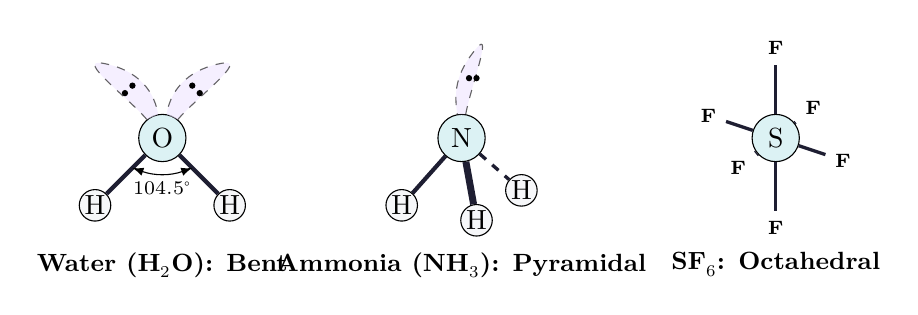
\begin{tikzpicture}[scale=0.95]
  % --- Water (Bent) ---
  \begin{scope}[xshift=-4.0cm, yshift=1.5cm]
    \node[draw, circle, fill=hdrteal, minimum size=0.6cm, inner sep=0pt] (O) at (0,0) {O};
    \node[draw, circle, fill=mygray, minimum size=0.4cm, inner sep=0pt] (H1) at (-0.9,-0.9) {H};
    \node[draw, circle, fill=mygray, minimum size=0.4cm, inner sep=0pt] (H2) at (0.9,-0.9) {H};
    
    \draw[line width=1.5pt, color=mydark] (O) -- (H1);
    \draw[line width=1.5pt, color=mydark] (O) -- (H2);
    
    % Draw lone pair lobes
    \draw[dashed, fill=hdrpurple, opacity=0.6] (O) to[out=50,in=10] (0.8,1.0) to[out=190,in=80] (O);
    \draw[dashed, fill=hdrpurple, opacity=0.6] (O) to[out=130,in=170] (-0.8,1.0) to[out=350,in=100] (O);
    \fill (0.4,0.7) circle (1.2pt); \fill (0.5,0.6) circle (1.2pt);
    \fill (-0.4,0.7) circle (1.2pt); \fill (-0.5,0.6) circle (1.2pt);
    
    % Angle label
    \draw[latex-latex, thin] (-0.4,-0.4) to[bend right=20] (0.4,-0.4);
    \node[below, font=\scriptsize] at (0,-0.45) {$104.5^\circ$};
    \node[below, font=\small\bfseries] at (0,-1.4) {Water ($\text{H}_2\text{O}$): Bent};
  \end{scope}

  % --- Ammonia (Trigonal Pyramidal) ---
  \begin{scope}[xshift=0.0cm, yshift=1.5cm]
    \node[draw, circle, fill=hdrteal, minimum size=0.6cm, inner sep=0pt] (N) at (0,0) {N};
    \node[draw, circle, fill=mygray, minimum size=0.4cm, inner sep=0pt] (H1) at (-0.8,-0.9) {H};
    \node[draw, circle, fill=mygray, minimum size=0.4cm, inner sep=0pt] (H2) at (0.2,-1.1) {H};
    \node[draw, circle, fill=mygray, minimum size=0.4cm, inner sep=0pt] (H3) at (0.8,-0.7) {H};
    
    \draw[line width=1.5pt, color=mydark] (N) -- (H1);
    \draw[line width=2.5pt, color=mydark] (N) -- (H2); % Wedged
    \draw[dashed, line width=1.2pt, color=mydark] (N) -- (H3); % Dashed
    
    % Lone pair lobe
    \draw[dashed, fill=hdrpurple, opacity=0.6] (N) to[out=80,in=50] (0.2,1.2) to[out=230,in=100] (N);
    \fill (0.1,0.8) circle (1.2pt); \fill (0.2,0.8) circle (1.2pt);
    
    \node[below, font=\small\bfseries] at (0,-1.4) {Ammonia ($\text{NH}_3$): Pyramidal};
  \end{scope}

  % --- Sulfur Hexafluoride (Octahedral) ---
  \begin{scope}[xshift=4.2cm, yshift=1.5cm]
    \node[draw, circle, fill=hdrteal, minimum size=0.6cm, inner sep=0pt] (S) at (0,0) {S};
    \node[font=\scriptsize\bfseries] (F1) at (0,1.2) {F};
    \node[font=\scriptsize\bfseries] (F2) at (0,-1.2) {F};
    \node[font=\scriptsize\bfseries] (F3) at (-0.9,0.3) {F};
    \node[font=\scriptsize\bfseries] (F4) at (0.9,-0.3) {F};
    \node[font=\scriptsize\bfseries] (F5) at (-0.5,-0.4) {F};
    \node[font=\scriptsize\bfseries] (F6) at (0.5,0.4) {F};
    
    \draw[line width=1.2pt, color=mydark] (S) -- (F1);
    \draw[line width=1.2pt, color=mydark] (S) -- (F2);
    \draw[line width=1.2pt, color=mydark] (S) -- (F3);
    \draw[line width=1.2pt, color=mydark] (S) -- (F4);
    \draw[line width=2.2pt, color=mydark] (S) -- (F5); % Wedged
    \draw[dashed, line width=1.2pt, color=mydark] (S) -- (F6); % Dashed
    
    \node[below, font=\small\bfseries] at (0,-1.4) {$\text{SF}_6$: Octahedral};
  \end{scope}
\end{tikzpicture}
\par\vspace{4pt}
\small\color{mydark}
3D orbital and bonding representations of tetrahedral-based shapes ($\text{H}_2\text{O}$ with 2 lone pairs; $\text{NH}_3$ with 1 lone pair) and octahedral geometry ($\text{SF}_6$ with 6 equivalent bonding directions).
\end{center}
\end{tcolorbox}

\textbf{4. Sulfur Tetrafluoride ($\text{SF}_4$): $sp^3d$ Hybridization, Seesaw Shape}
\begin{itemize}[leftmargin=*, itemsep=1pt]
  \item Central atom: Sulfur ($[\text{Ne}]3s^2 3p^4$). It has 6 valence electrons.
  \item Bonds: 4 single bonds with Fluorine, sharing 4 electrons.
  \item Electron pairs: $\text{SN} = 4\text{ (bp)} + 1\text{ (lp)} = 5$ electron pairs.
  \item Geometry: Based on a trigonal bipyramid. The single lone pair can occupy either an axial position or an equatorial position:
    \begin{itemize}
      \item \textbf{Axial lone pair:} Experiences three $90^\circ$ lone pair-bonding pair repulsions.
      \item \textbf{Equatorial lone pair:} Experiences only two $90^\circ$ lone pair-bonding pair repulsions.
    \end{itemize}
    To minimize electrostatic repulsions, the lone pair occupies the roomier \textbf{equatorial position}. The resulting shape is called a \textbf{Seesaw}.
  \item Distortion: The equatorial lone pair repels the axial and equatorial $\text{S-F}$ bonds, compressing the axial $\text{F-S-F}$ angle from $180^\circ$ to $173^\circ$, and the equatorial $\text{F-S-F}$ angle from $120^\circ$ to $101.5^\circ$.
\end{itemize}

\textbf{5. Chlorine Trifluoride ($\text{ClF}_3$): $sp^3d$ Hybridization, T-shaped Shape}
\begin{itemize}[leftmargin=*, itemsep=1pt]
  \item Central atom: Chlorine ($[\text{Ne}]3s^2 3p^5$). It has 7 valence electrons.
  \item Bonds: 3 single bonds with Fluorine, sharing 3 electrons.
  \item Electron pairs: $\text{SN} = 3\text{ (bp)} + 2\text{ (lp)} = 5$ electron pairs.
  \item Geometry: Based on a trigonal bipyramid. To minimize repulsions, both lone pairs occupy the \textbf{equatorial positions}. The three Fluorine atoms occupy the two axial and one equatorial positions, yielding a \textbf{T-shaped} molecule.
  \item Distortion: The two equatorial lone pairs exert strong repulsions, bending the axial $\text{F-Cl-F}$ bond axis slightly towards the equatorial Fluorine atom, compressing the axial-equatorial angles from $90^\circ$ to $87.5^\circ$.
\end{itemize}

\textbf{6. Xenon Difluoride ($\text{XeF}_2$): $sp^3d$ Hybridization, Linear Shape}
\begin{itemize}[leftmargin=*, itemsep=1pt]
  \item Central atom: Xenon ($5s^2 5p^6$). It has 8 valence electrons.
  \item Bonds: 2 single bonds with Fluorine, sharing 2 electrons.
  \item Electron pairs: $\text{SN} = 2\text{ (bp)} + 3\text{ (lp)} = 5$ electron pairs.
  \item Geometry: Based on a trigonal bipyramid. All three lone pairs occupy the three \textbf{equatorial positions} where they lie at $120^\circ$ to each other, cancelling their electrostatic repulsions. The two Fluorine atoms occupy the two axial positions. The molecular shape is perfectly \textbf{Linear} ($\text{F-Xe-F}$ bond angle $= 180^\circ$).
\end{itemize}

\textbf{7. Xenon Tetrafluoride ($\text{XeF}_4$): $sp^3d^2$ Hybridization, Square Planar Shape}
\begin{itemize}[leftmargin=*, itemsep=1pt]
  \item Central atom: Xenon ($5s^2 5p^6$). It has 8 valence electrons.
  \item Bonds: 4 single bonds with Fluorine, sharing 4 electrons.
  \item Electron pairs: $\text{SN} = 4\text{ (bp)} + 2\text{ (lp)} = 6$ electron pairs.
  \item Geometry: Based on an octahedron. The two lone pairs can be placed adjacent ($90^\circ$) or opposite ($180^\circ$) to each other.
    To minimize the strong lone pair-lone pair repulsion, the two lone pairs occupy the \textbf{axial positions} opposite each other ($180^\circ$). The four Fluorine atoms occupy the equatorial positions, yielding a symmetric \textbf{Square Planar} geometry (bond angles $= 90^\circ$).
\end{itemize}

\begin{tcolorbox}[tikzbox, title={VSEPR Geometries (Part B): Trigonal Bipyramidal-based shapes}]
\begin{center}
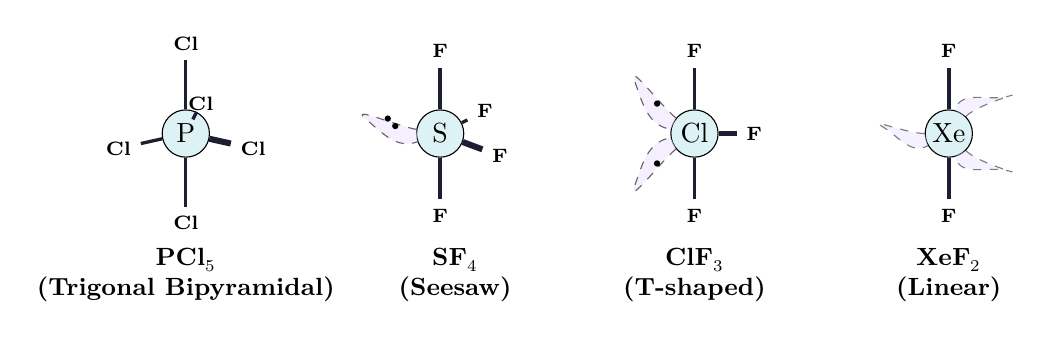
\begin{tikzpicture}[scale=0.95]
  % --- PCl5 (Trigonal Bipyramidal) ---
  \begin{scope}[xshift=-5.1cm]
    \node[draw, circle, fill=hdrteal, minimum size=0.6cm, inner sep=0pt] (P) at (0,0) {P};
    \node[font=\scriptsize\bfseries] (Cl1) at (0,1.2) {Cl};
    \node[font=\scriptsize\bfseries] (Cl2) at (0,-1.2) {Cl};
    \node[font=\scriptsize\bfseries] (Cl3) at (-0.9,-0.2) {Cl};
    \node[font=\scriptsize\bfseries] (Cl4) at (0.9,-0.2) {Cl};
    \node[font=\scriptsize\bfseries] (Cl5) at (0.2,0.4) {Cl};
    
    \draw[line width=1.2pt, color=mydark] (P) -- (Cl1);
    \draw[line width=1.2pt, color=mydark] (P) -- (Cl2);
    \draw[line width=1.2pt, color=mydark] (P) -- (Cl3);
    \draw[line width=2.2pt, color=mydark] (P) -- (Cl4); % Wedged
    \draw[dashed, line width=1.2pt, color=mydark] (P) -- (Cl5); % Dashed
    
    \node[below, font=\small\bfseries, align=center] at (0,-1.4) {$\text{PCl}_5$ \\ (Trigonal Bipyramidal)};
  \end{scope}

  % --- SF4 (Seesaw) ---
  \begin{scope}[xshift=-1.7cm]
    \node[draw, circle, fill=hdrteal, minimum size=0.6cm, inner sep=0pt] (S) at (0,0) {S};
    \node[font=\scriptsize\bfseries] (F1) at (0,1.1) {F};
    \node[font=\scriptsize\bfseries] (F2) at (0,-1.1) {F};
    \node[font=\scriptsize\bfseries] (F3) at (0.8,-0.3) {F};
    \node[font=\scriptsize\bfseries] (F4) at (0.6,0.3) {F};
    
    \draw[line width=1.2pt, color=mydark] (S) -- (F1);
    \draw[line width=1.2pt, color=mydark] (S) -- (F2);
    \draw[line width=2.2pt, color=mydark] (S) -- (F3); % Wedged
    \draw[dashed, line width=1.2pt, color=mydark] (S) -- (F4); % Dashed
    
    % Equatorial lone pair lobe
    \draw[dashed, fill=hdrpurple, opacity=0.6] (S) to[out=170,in=140] (-1.0,0.2) to[out=320,in=200] (S);
    \fill (-0.6,0.1) circle (1.2pt); \fill (-0.7,0.2) circle (1.2pt);
    
    \node[below, font=\small\bfseries, align=center] at (0.2,-1.4) {$\text{SF}_4$ \\ (Seesaw)};
  \end{scope}

  % --- ClF3 (T-shaped) ---
  \begin{scope}[xshift=1.7cm]
    \node[draw, circle, fill=hdrteal, minimum size=0.6cm, inner sep=0pt] (Cl) at (0,0) {Cl};
    \node[font=\scriptsize\bfseries] (F1) at (0,1.1) {F};
    \node[font=\scriptsize\bfseries] (F2) at (0,-1.1) {F};
    \node[font=\scriptsize\bfseries] (F3) at (0.8,0.0) {F};
    
    \draw[line width=1.2pt, color=mydark] (Cl) -- (F1);
    \draw[line width=1.2pt, color=mydark] (Cl) -- (F2);
    \draw[line width=1.5pt, color=mydark] (Cl) -- (F3);
    
    % Two equatorial lone pairs
    \draw[dashed, fill=hdrpurple, opacity=0.6] (Cl) to[out=140,in=110] (-0.8,0.7) to[out=290,in=170] (Cl);
    \draw[dashed, fill=hdrpurple, opacity=0.6] (Cl) to[out=220,in=250] (-0.8,-0.7) to[out=70,in=190] (Cl);
    \fill (-0.5,0.4) circle (1.2pt); \fill (-0.5,-0.4) circle (1.2pt);
    
    \node[below, font=\small\bfseries, align=center] at (0,-1.4) {$\text{ClF}_3$ \\ (T-shaped)};
  \end{scope}

  % --- XeF2 (Linear) ---
  \begin{scope}[xshift=5.1cm]
    \node[draw, circle, fill=hdrteal, minimum size=0.6cm, inner sep=0pt] (Xe) at (0,0) {Xe};
    \node[font=\scriptsize\bfseries] (F1) at (0,1.1) {F};
    \node[font=\scriptsize\bfseries] (F2) at (0,-1.1) {F};
    
    \draw[line width=1.5pt, color=mydark] (Xe) -- (F1);
    \draw[line width=1.5pt, color=mydark] (Xe) -- (F2);
    
    % Three equatorial lone pairs
    \draw[dashed, fill=hdrpurple, opacity=0.5] (Xe) to[out=180,in=150] (-0.9,0.1) to[out=330,in=210] (Xe);
    \draw[dashed, fill=hdrpurple, opacity=0.5] (Xe) to[out=45,in=15] (0.8,0.5) to[out=195,in=75] (Xe);
    \draw[dashed, fill=hdrpurple, opacity=0.5] (Xe) to[out=-45,in=-15] (0.8,-0.5) to[out=165,in=-75] (Xe);
    
    \node[below, font=\small\bfseries, align=center] at (0,-1.4) {$\text{XeF}_2$ \\ (Linear)};
  \end{scope}
\end{tikzpicture}
\par\vspace{4pt}
\small\color{mydark}
The evolution of shapes within the Steric Number 5 family ($\text{PCl}_5, \text{SF}_4, \text{ClF}_3, \text{XeF}_2$). Note that lone pairs always preferentially occupy the equatorial positions to minimize close $90^\circ$ repulsions.
\end{center}
\end{tcolorbox}

\subsection{Summary of SN and Molecular Shapes}
\par\vspace{4pt}\noindent
\begin{tabularx}{\linewidth}{|B{1.6cm}|B{2.2cm}|B{2.0cm}|B{2.8cm}|Y|}
\hline
\textbf{SN} & \textbf{Bond Pairs} & \textbf{Lone Pairs} & \textbf{Molecular Shape} & \textbf{Example} \\
\hline
\textbf{2} & 2 & 0 & Linear & $\text{CO}_2$, $\text{BeCl}_2$ \\
\hline
\multirow{2}{*}{\textbf{3}} & 3 & 0 & Trigonal Planar & $\text{BF}_3$, $\text{AlCl}_3$ \\
\cline{2-5}
 & 2 & 1 & Bent (V-shaped) & $\text{SO}_2$, $\text{O}_3$ \\
\hline
\multirow{3}{*}{\textbf{4}} & 4 & 0 & Tetrahedral & $\text{CH}_4$, $\text{SiCl}_4$ \\
\cline{2-5}
 & 3 & 1 & Trigonal Pyramidal & $\text{NH}_3$, $\text{PH}_3$ \\
\cline{2-5}
 & 2 & 2 & Bent (V-shaped) & $\text{H}_2\text{O}$, $\text{OF}_2$ \\
\hline
\multirow{4}{*}{\textbf{5}} & 5 & 0 & Trigonal Bipyramidal & $\text{PCl}_5$, $\text{SbF}_5$ \\
\cline{2-5}
 & 4 & 1 & Seesaw & $\text{SF}_4$, $\text{SeF}_4$ \\
\cline{2-5}
 & 3 & 2 & T-shaped & $\text{ClF}_3$, $\text{ICl}_3$ \\
\cline{2-5}
 & 2 & 3 & Linear & $\text{XeF}_2$, $\text{I}_3^-$ \\
\hline
\multirow{3}{*}{\textbf{6}} & 6 & 0 & Octahedral & $\text{SF}_6$, $\text{SeF}_6$ \\
\cline{2-5}
 & 5 & 1 & Square Pyramidal & $\text{BrF}_5$, $\text{IF}_5$ \\
\cline{2-5}
 & 4 & 2 & Square Planar & $\text{XeF}_4$, $\text{ICl}_4^-$ \\
\hline
\end{tabularx}
\vspace{6pt}

\begin{tcolorbox}[exambox, title={Exam Points: VSEPR and Shapes}]
  \begin{itemize}[leftmargin=*, itemsep=2pt, topsep=2pt]
    \item \textbf{Postulates:} State Gillespie-Nyholm rules clearly, emphasizing $\text{lp-lp} > \text{lp-bp} > \text{bp-bp}$ repulsion hierarchy.
    \item \textbf{Bond Angle Distortions:} Explain the angles of $\text{H}_2\text{O}$ ($104.5^\circ$) and $\text{NH}_3$ ($107^\circ$) by referencing lone pair repulsions.
    \item \textbf{Trigonal Bipyramid rule:} State clearly that lone pairs must occupy the equatorial positions first.
    \item \textbf{Bond length inequality in $\text{PCl}_5$:} Explain why axial bonds are longer than equatorial ones by counting $90^\circ$ repulsions.
    \item \textbf{Square Planar $\text{XeF}_4$:} Explain why the lone pairs occupy axial positions ($180^\circ$ apart) to minimize lp-lp repulsion.
  \end{itemize}
\end{tcolorbox}

\newpage
\begin{center}
  {\large\bfseries\color{myred} Quick Revision --- Module 5}\\[3pt]
  {\small\color{mydark} Periodic Properties $|$ BS-CH101}
\end{center}
\noindent{\color{myred}\rule{\linewidth}{1.2pt}}
\vspace{4pt}

\begin{tcolorbox}[formulabox, breakable, title={Key Formulas at a Glance},
  title after break={\textbf{Key Formulas at a Glance (contd.)}}]
\renewcommand{\arraystretch}{1.55}
\begin{tabularx}{\linewidth}{|B{4.5cm}|Y|}
\hline
\textbf{Formula} & \textbf{Meaning} \\
\hline
$Z_{\text{eff}} = Z - \sigma$ & Effective Nuclear Charge. \\
\hline
$\sigma = (n_{\text{same}} \times 0.35) + (n_{n-1} \times 0.85) + (n_{\text{inner}} \times 1.00)$ & Slater's rule for valence $(ns, np)$ electrons (except $1s$: $\sigma = 0.30$). \\
\hline
$\sigma = (n_{\text{same}} \times 0.35) + (n_{\text{left}} \times 1.00)$ & Slater's rule for $(nd)$ or $(nf)$ valence electrons. \\
\hline
$N_r = n - l - 1$ & Radial (spherical) nodes. \\
\hline
$N_a = l$ & Angular nodes (nodal planes). \\
\hline
$N_{\text{total}} = n - 1$ & Total nodes. \\
\hline
$P = \displaystyle\frac{n(n-1)}{2}$ & Hund's rule: possible exchange count for $n$ parallel-spin electrons. \\
\hline
$\chi_A - \chi_B = 0.102 \sqrt{\Delta}$ & Pauling electronegativity difference ($\Delta$ in $\text{kJ\,mol}^{-1}$). \\
\hline
$\Delta = E_{AB} - \sqrt{E_{AA} \cdot E_{BB}}$ & Pauling's ionic resonance stabilization energy. \\
\hline
$\chi_{\text{M}} = \displaystyle\frac{\text{IE} + \text{EA}}{2}$ & Mulliken electronegativity ($\text{IE}$, $\text{EA}$ in $\text{eV}$). \\
\hline
$\chi_{\text{P}} \approx \displaystyle\frac{\text{IE(eV)} + \text{EA(eV)}}{5.6}$ & Mulliken-to-Pauling electronegativity scale conversion. \\
\hline
$\chi_{\text{P}} \approx \displaystyle\frac{\text{IE} + \text{EA}}{540}$ & Mulliken-to-Pauling conversion ($\text{IE}$, $\text{EA}$ in $\text{kJ\,mol}^{-1}$). \\
\hline
$\chi_{\text{AR}} = 0.359 \displaystyle\frac{Z_{\text{eff}}}{r^2} + 0.744$ & Allred-Rochow electronegativity ($r$ in \text{\AA}). \\
\hline
$\% \text{ Ionic Character} = 16 |\chi_A - \chi_B| + 3.5 |\chi_A - \chi_B|^2$ & Hannay-Smith equation. \\
\hline
$\% \text{ Ionic Character} = 100 \left(1 - e^{-0.25(\chi_A - \chi_B)^2}\right)$ & Pauling's ionic character formula. \\
\hline
$\eta = \displaystyle\frac{I - A}{2}$ & DFT Chemical Hardness ($I = \text{IE}$, $A = \text{EA}$). \\
\hline
$S = \displaystyle\frac{1}{\eta} = \displaystyle\frac{2}{I - A}$ & DFT Chemical Softness. \\
\hline
$\text{SN} = \text{Bonded Atoms} + \text{Lone Pairs}$ & Steric Number for VSEPR/hybridization. \\
\hline
$\phi = \displaystyle\frac{q}{r}$ & Ionic potential (charge density) for Fajans' polarization. \\
\hline
\end{tabularx}
\end{tcolorbox}

\begin{tcolorbox}[defbox, title={One-Line Definitions}]
\begin{itemize}[leftmargin=*, itemsep=2.pt, topsep=2pt]
  \item \textbf{Shielding effect:} The screening of outer electrons from nuclear attraction by inner electrons.
  \item \textbf{Effective nuclear charge ($Z_{\text{eff}}$):} The net positive charge experienced by an electron in a multi-electron atom.
  \item \textbf{Penetration power:} The relative probability density of finding an orbital's electron close to the nucleus.
  \item \textbf{Radial node:} A spherical surface around the nucleus where the electron probability density is zero.
  \item \textbf{Aufbau principle:} The rule stating that electrons fill subshells in order of increasing $(n+l)$ energy.
  \item \textbf{Pauli exclusion principle:} A rule stating that no two electrons in an atom can have the same four quantum numbers.
  \item \textbf{Hund's rule:} Degenerate orbitals are filled singly with parallel spins before electron pairing begins.
  \item \textbf{Exchange energy:} The electrostatic stabilization energy released when parallel-spin electrons swap degenerate positions.
  \item \textbf{Covalent radius:} One-half of the distance between the nuclei of two identical single-bonded atoms.
  \item \textbf{Metallic radius:} One-half of the distance between adjacent metal cations in a crystal lattice.
  \item \textbf{Van der Waals radius:} One-half of the closest distance between non-bonded adjacent atoms in a solid lattice.
  \item \textbf{Ionic radius:} The effective distance from an ion's nucleus where it exerts electrostatic control over its electron cloud.
  \item \textbf{Lanthanide contraction:} The steady contraction in atomic and ionic radii along the lanthanide series ($La \to Lu$).
  \item \textbf{Isoelectronic species:} Atoms or ions sharing the same number and distribution of electrons.
  \item \textbf{Ionization energy:} The minimum energy required to remove the most loosely bound electron from a gaseous atom.
  \item \textbf{Successive ionization energies:} Energies required to remove further electrons sequentially ($IE_1 < IE_2 < IE_3 \dots$).
  \item \textbf{Electron affinity:} The energy released when an electron is added to a neutral gaseous atom.
  \item \textbf{Electron gain enthalpy ($\Delta_{\text{eg}}H$):} The enthalpy change accompanying the addition of an electron to an atom.
  \item \textbf{Electronegativity:} The tendency of an atom in a molecule to attract the shared bonding electron pair.
  \item \textbf{Polarizing power:} The ability of a cation to distort the electron cloud of an adjacent anion.
  \item \textbf{Polarizability:} The susceptibility of an anion's electron cloud to distortion by a cation.
  \item \textbf{Fajans' rules:} A set of empirical rules predicting the degree of covalent character in an ionic bond.
  \item \textbf{Pseudo-noble gas configuration:} Cation valence configurations with 18 electrons ($ns^2 np^6 nd^{10}$).
  \item \textbf{Oxidation state:} The formal charge an atom would carry if all bonds were purely ionic.
  \item \textbf{Coordination number:} The number of donor atoms directly bonded to a central metal ion.
  \item \textbf{Coordination geometry:} The spatial arrangement of coordinating ligands around the central metal ion.
  \item \textbf{Inert pair effect:} The reluctance of the outermost valence $ns^2$ pair to participate in chemical bonding in heavier post-transition metals.
  \item \textbf{Hard acid/base:} Cations/anions of small size and low polarizability.
  \item \textbf{Soft acid/base:} Cations/anions of large size and high polarizability.
  \item \textbf{Steric number:} The sum of bonded atoms and lone pairs around a central atom in VSEPR theory.
\end{itemize}
\end{tcolorbox}

\begin{tcolorbox}[exambox, title={Frequently Asked / Viva Questions}]
  \Q{Q1. Why is the first ionization energy of Nitrogen greater than that of Oxygen?}
  Nitrogen has a stable, half-filled $2p^3$ subshell ($2p_x^1 2p_y^1 2p_z^1$) which possesses high exchange energy. Oxygen has $2p^4$, containing a paired electron in the $2p_x$ orbital. The inter-electronic repulsion between these paired electrons makes it easier to remove an electron from Oxygen, resulting in $IE_1(\text{N}) > IE_1(\text{O})$.
  \par\vspace{6pt}
  \Q{Q2. Why does Chlorine have a higher electron affinity than Fluorine?}
  Fluorine is extremely small, and its valence electrons occupy a highly compact $2p$ subshell. Adding an electron to this small volume causes intense inter-electronic repulsion, which offsets some of the energy released. Chlorine is larger and its diffuse $3p$ subshell accommodates the incoming electron with much less repulsion, releasing more net energy.
  \par\vspace{6pt}
  \Q{Q3. What is the cause of the Lanthanide Contraction?}
  The addition of electrons to the inner $4f$ subshell. The $4f$ orbitals are diffuse and shield the increasing nuclear charge ($+1$ per element) very poorly. Consequently, the effective nuclear charge felt by outer electrons increases steadily, contracting the shell.
  \par\vspace{6pt}
  \Q{Q4. Explain why Zirconium ($\text{Zr}$) and Hafnium ($\text{Hf}$) have almost identical atomic radii.}
  Hafnium ($5d$, $Z=72$) follows the lanthanides ($La \to Lu$). The intervening 14 lanthanide elements undergo a steady atomic shrinkage (lanthanide contraction). This shrinkage cancels out the normal size increase expected from adding a new principal shell, making $r_{\text{Zr}} \approx r_{\text{Hf}}$.
  \par\vspace{6pt}
  \Q{Q5. Why is the first ionization energy of Beryllium greater than that of Boron?}
  Beryllium ($1s^2 2s^2$) has a fully-filled $2s$ subshell. The valence electron is removed from a $2s$ orbital, which is more penetrating and bound tighter than the $2p$ valence electron in Boron ($1s^2 2s^2 2p^1$).
  \par\vspace{6pt}
  \Q{Q6. State Fajans' rules for covalent character in ionic compounds.}
  Covalent character increases with: (i) small cation size, (ii) large anion size, (iii) high charges on the ions, and (iv) pseudo-noble gas configurations ($ns^2 np^6 nd^{10}$) of the cation.
  \par\vspace{6pt}
  \Q{Q7. Explain why $\text{CuCl}$ is insoluble in water whereas $\text{NaCl}$ is soluble.}
  $\text{Cu}^+$ has a pseudo-noble gas configuration ($3d^{10}$). The $d$-electrons shield the nucleus poorly, giving $\text{Cu}^+$ a higher polarizing power than $\text{Na}^+$ (noble gas configuration). This strong polarization introduces covalent character in $\text{CuCl}$, making it insoluble in water.
  \par\vspace{6pt}
  \Q{Q8. What is the inert pair effect?}
  The reluctance of the outermost $ns^2$ valence pair to participate in chemical bonding in heavier post-transition elements of Groups 13-15 (Tl, Pb, Bi) due to poor shielding by $d/f$ subshells and valence shell contraction.
  \par\vspace{6pt}
  \Q{Q9. Why is $\text{PbO}_2$ a strong oxidizing agent while $\text{PbO}$ is stable?}
  Due to the inert pair effect, the stable oxidation state for Lead is $+2$. Lead in the $+4$ state ($\text{PbO}_2$) is unstable and acts as a powerful oxidizing agent to reduce itself to the stable $+2$ state ($\text{Pb}^{2+}$).
  \par\vspace{6pt}
  \Q{Q10. State the Pearson HSAB principle.}
  Hard acids prefer to coordinate with hard bases (forming stable ionic bonds), and soft acids prefer to coordinate with soft bases (forming stable covalent bonds).
  \par\vspace{6pt}
  \Q{Q11. Explain why calcium occurs as $\text{CaCO}_3$ in nature but copper occurs as $\text{Cu}_2\text{S}$.}
  $\text{Ca}^{2+}$ is a hard acid and coordinates stably with the hard base carbonate ($\text{CO}_3^{2-}$). $\text{Cu}^+$ is a soft acid and coordinates stably with the soft base sulfide ($\text{S}^{2-}$).
  \par\vspace{6pt}
  \Q{Q12. Why is $\text{AgI}$ insoluble in water but $\text{AgF}$ is soluble?}
  $\text{Ag}^+$ and $\text{I}^-$ are both soft. The soft-soft covalent lattice in $\text{AgI}$ is highly stable and cannot be broken by the hard solvent water. In $\text{AgF}$, the mismatched hard-soft interaction is weak, and the hard $\text{F}^-$ is strongly hydrated, driving dissolution.
  \par\vspace{6pt}
  \Q{Q13. State the postulates of VSEPR theory.}
  Valence electron pairs (bonding and lone pairs) around a central atom repel each other and orient in space to maximize distance and minimize repulsion.
  \par\vspace{6pt}
  \Q{Q14. What is the order of repulsive forces between electron pairs in VSEPR?}
  $\text{Lone Pair -- Lone Pair (lp-lp)} > \text{Lone Pair -- Bonding Pair (lp-bp)} > \text{Bonding Pair -- Bonding Pair (bp-bp)}$.
  \par\vspace{6pt}
  \Q{Q15. Why is the bond angle of $\text{H}_2\text{O}$ ($104.5^\circ$) smaller than that of $\text{NH}_3$ ($107^\circ$)?}
  Water has two lone pairs on Oxygen which repel each other and compress the bonding pairs strongly. Ammonia has only one lone pair on Nitrogen, which exerts less compressive repulsion.
  \par\vspace{6pt}
  \Q{Q16. Why are the axial $\text{P-Cl}$ bonds in $\text{PCl}_5$ longer than the equatorial ones?}
  The two axial chlorine atoms experience stronger electrostatic repulsions from the three equatorial chlorine atoms at $90^\circ$, forcing the axial bonds to lengthen to minimize repulsions.
  \par\vspace{6pt}
  \Q{Q17. What is the shape of $\text{SF}_4$?}
  Seesaw. The lone pair occupies an equatorial position to minimize $90^\circ$ repulsions (it experiences only two $90^\circ$ repulsions, compared to three if it were axial).
  \par\vspace{6pt}
  \Q{Q18. What are isoelectronic species? Give an example.}
  Atoms or ions containing the same number of electrons. Example: $\text{N}^{3-}, \text{O}^{2-}, \text{F}^-, \text{Na}^+, \text{Mg}^{2+}$, all of which have 10 electrons.
  \par\vspace{6pt}
  \Q{Q19. Why does ionic radius increase with coordination number?}
  A higher coordination number requires the central ion to expand its coordination sphere to accommodate more ligands, reducing steric repulsions and effectively increasing its radius.
  \par\vspace{6pt}
  \Q{Q20. Write the Slater's rules groupings.}
  $(1s) \; (2s, 2p) \; (3s, 3p) \; (3d) \; (4s, 4p) \; (4d) \; (4f) \; (5s, 5p) \; (5d) \dots$
  \par\vspace{6pt}
  \Q{Q21. Why are $s$-electrons more penetrating than $p$-electrons?}
  The angular momentum barrier is zero for $s$-orbitals ($l=0$). This allows the radial wavefunction of $s$-orbitals to have significant density peaks very close to the nucleus.
  \par\vspace{6pt}
  \Q{Q22. Define chemical hardness and write its operational formula.}
  Resistance of a chemical species to charge transfer and polarization. Formula: $\eta = (I-A)/2$.
  \par\vspace{6pt}
  \Q{Q23. Why do noble gases have positive electron gain enthalpies?}
  Noble gases have stable, closed-shell configurations ($ns^2 np^6$). Adding an electron requires forcing it into a higher principal energy shell ($n+1$), which is highly endothermic.
  \par\vspace{6pt}
  \Q{Q24. Why is $\text{ClF}_3$ T-shaped and not trigonal planar?}
  The central Chlorine has 5 electron pairs ($\text{SN} = 5$). To minimize repulsions, the two lone pairs occupy equatorial positions, leaving the three Fluorine atoms to form a T-shape.
  \par\vspace{6pt}
  \Q{Q25. Why is $\text{XeF}_4$ square planar?}
  Xenon has 6 electron pairs ($\text{SN} = 6$). The two lone pairs occupy axial positions directly opposite each other ($180^\circ$ apart) to minimize repulsions, leaving the four fluorines in a square plane.
  \par\vspace{6pt}
  \Q{Q26. Why does electronegativity increase across a period?}
  As nuclear charge increases and atomic size contracts, the nucleus can exert a stronger electrostatic pull on bonding electron pairs.
  \par\vspace{6pt}
  \Q{Q27. How does the Allred-Rochow scale calculate electronegativity?}
  Based on the electrostatic force of attraction: $\chi_{\text{AR}} = 0.359 (Z_{\text{eff}}/r^2) + 0.744$.
  \par\vspace{6pt}
  \Q{Q28. What is the significance of the Hannay-Smith equation?}
  It calculates the percentage of ionic character in a polar covalent bond from electronegativity differences: $\% = 16\Delta\chi + 3.5\Delta\chi^2$.
  \par\vspace{6pt}
  \Q{Q29. What is orbital collapse?}
  The sudden, rapid stabilization and drop in energy of $d$ or $f$ orbitals as nuclear charge increases, occurring when those shells begin to fill.
  \par\vspace{6pt}
  \Q{Q30. What is exchange energy and how does it stabilize half-filled orbitals?}
  It is the stabilization energy released when electrons of parallel spin swap degenerate orbital positions. Half-filled shells have maximum possible parallel-spin pairs, maximizing exchanges.
\end{tcolorbox}

\begin{tcolorbox}[tikzbox, title={Summary of Periodic Trends}]
\renewcommand{\arraystretch}{1.55}
\begin{tabularx}{\linewidth}{|B{3.2cm}|Y|Y|Y|}
\hline
\textbf{Property} & \textbf{Definition} & \textbf{Trend (Across Period)} & \textbf{Trend (Down Group)} \\
\hline
\textbf{Effective Nuclear Charge ($Z_{\text{eff}}$)} & Net positive charge felt by valence electrons. & Increases (by $+0.65$ per element) & Remains relatively constant or increases slightly \\
\hline
\textbf{Atomic Size ($r$)} & Bonding or non-bonding atomic boundary. & Decreases (stronger nuclear pull) & Increases (new shells added) \\
\hline
\textbf{Ionization Energy (IE)} & Energy required to remove valence electron. & Increases (valence shell bound tighter) & Decreases (outer electron farther away) \\
\hline
\textbf{Electron Affinity (EA)} & Energy released upon gaining valence electron. & Becomes more positive (except noble gases) & Generally decreases \\
\hline
\textbf{Electronegativity ($\chi$)} & Pull on shared bonding electron pairs. & Increases & Decreases \\
\hline
\end{tabularx}
\end{tcolorbox}

\end{document}


